%%%%%%%%%%%%%%%%%%%%%%%%%%%%%%%%%%%%%%%%%
% The Legrand Orange Book
% LaTeX Template
% Version 2.1.1 (14/2/16)
%
% This template has been downloaded from:
% http://www.LaTeXTemplates.com
%
% Original author:
% Mathias Legrand (legrand.mathias@gmail.com) with modifications by:
% Vel (vel@latextemplates.com)
%
% License:
% CC BY-NC-SA 3.0 (http://creativecommons.org/licenses/by-nc-sa/3.0/)
%
% Compiling this template:
% This template uses biber for its bibliography and makeindex for its index.
% When you first open the template, compile it from the command line with the
% commands below to make sure your LaTeX distribution is configured correctly:
%
% 1) pdflatex main
% 2) makeindex main.idx -s StyleInd.ist
% 3) biber main
% 4) pdflatex main x 2
%
% After this, when you wish to update the bibliography/index use the appropriate
% command above and make sure to compile with pdflatex several times
% afterwards to propagate your changes to the document.
%
% This template also uses a number of packages which may need to be
% updated to the newest versions for the template to compile. It is strongly
% recommended you update your LaTeX distribution if you have any
% compilation errors.
%
% Important note:
% Chapter heading images should have a 2:1 width:height ratio,
% e.g. 920px width and 460px height.
%
%%%%%%%%%%%%%%%%%%%%%%%%%%%%%%%%%%%%%%%%%

%----------------------------------------------------------------------------------------
%	PACKAGES AND OTHER DOCUMENT CONFIGURATIONS
%----------------------------------------------------------------------------------------

\documentclass[11pt,oneside]{book} % Default font size and left-justified equations

%----------------------------------------------------------------------------------------

\input{structure} % Insert the commands.tex file which contains the majority of the structure behind the template

\begin{document}

%----------------------------------------------------------------------------------------
%	TITLE PAGE
%----------------------------------------------------------------------------------------

\begingroup
\thispagestyle{empty}
\begin{tikzpicture}[remember picture,overlay]
\coordinate [below=12cm] (midpoint) at (current page.north);
\node at (current page.north west)
{\begin{tikzpicture}[remember picture,overlay]
\node[anchor=north west,inner sep=0pt] at (0,0) {\includegraphics[width=\paperwidth]{background}}; % Background image
\draw[anchor=north] (midpoint) node [fill=hhublue!30!white,fill opacity=0.6,text opacity=1,inner sep=1cm]{\Huge\centering\bfseries\sffamily\parbox[c][][t]{\paperwidth}{\centering Grundlagen der künstlichen Intelligenz\\[15pt] % Book title
{\Large Vorlesungsskript}\\[20pt] % Subtitle
{\huge Sebastian Krings, et al.}}}; % Author name
\end{tikzpicture}};
\end{tikzpicture}
\vfill
\endgroup

%----------------------------------------------------------------------------------------
%	COPYRIGHT PAGE
%----------------------------------------------------------------------------------------

\newpage
\thispagestyle{empty}

\noindent This book and the corresponding slides are based on work of the students of our artifical intelligence course. We would like to thank all contributors.

\noindent
The contributors are (in alphabetical order):
\begin{itemize}
		\item Ahmadi, Sirat
    \item Batiukova, Olga
    \item Brenneis, Markus
    \item Brümmer, Ronny
		\item Dreyer, Kevin
    \item Funke, Andreas
    \item Happe, Chistopher
    \item Kerkmann, Anna Maria
    \item Komander, Dominique
    \item Krzysztala, Denis
    \item Michels, Daniel
    \item Moreira Hamasaki, Thaís
    \item Nalecz, Rafael
    \item Oberländer, Nils
    \item Özen, Eyyüp
    \item Papenberg, Martin
    \item Petrasch, Jessica
    \item Schmidt, Joshua
		\item Seliger, Kerstin
    \item Sura, Sebastian
    \item Thelen, Alexander
    \item Ullrich, Julian
    \item Weck, Sandy
    \item Weißenfeld, Anke Leonie
\end{itemize}

~\vfill

\noindent Copyright \copyright\ 2016-2017 Sebastian Krings, Michael Leuschel and others\\ % Copyright notice

%\noindent \textsc{Published by Publisher}\\ % Publisher

\noindent \url{http://www.stups.hhu.de}\\ % URL

\noindent
\begin{wrapfigure}[4]{l}[0cm]{0.0\textwidth}
%  \begin{center}
\includegraphics{images/creativecommons.png}
 % \end{center}
\end{wrapfigure}
 Licensed under the Creative Commons Attribution-NonCommercial-NoDerivatives 4.0 International Public License (the ``License''). You may not use this file except in compliance with the License. You may obtain a copy of the License at \url{http://creativecommons.org/licenses/by-nc-nd/4.0/}. Unless required by applicable law or agreed to in writing, software distributed under the License is distributed on an \textsc{``as is'' basis, without warranties or conditions of any kind}, either express or implied. See the License for the specific language governing permissions and limitations under the License.\\ % License information

%\noindent \textit{First printing, March 2013} % Printing/edition date

%----------------------------------------------------------------------------------------
%	TABLE OF CONTENTS
%----------------------------------------------------------------------------------------

%\usechapterimagefalse % If you don't want to include a chapter image, use this to toggle images off - it can be enabled later with \usechapterimagetrue

\chapterimage{chapter_head_1.png} % Table of contents heading image

\pagestyle{empty} % No headers

\tableofcontents % Print the table of contents itself

\cleardoublepage % Forces the first chapter to start on an odd page so it's on the right

\pagestyle{fancy} % Print headers again

\part{Einleitung}
bilder zu Forward Chaining


\part{Reasoning}
\chapterimage{chapter_head_1.png} % Chapter heading image

\chapter{Regelbasierte Expertensysteme}



%----------------------------------------------------------------------------------------
%	Einleitung
%----------------------------------------------------------------------------------------
\section{Einleitung}
Ein Expertensystem \textit{(kurz „XPS“)} ist ein Computerprogramm, welche das Wissen spezialisierter Fachleute nachbildet. Dadurch, dass sie das Wissen über einen spezifischen Sachbereich haben, können sie Experten bei ihren täglichen Aufgaben unterstützen und sind zudem in der Lage ihr Wissen jederzeit zur Verfügung zu stellen.

\begin{center}
    \textit{
        „Expertensysteme sind Programme, mit denen das Spezialwissen und die Schlußfolgerungsfähigkeit qualifizierter Fachleute auf eng begrenzten Aufgabengebieten nachgebildet werden soll.“
    }\cite{puppe}\\
\end{center}

\noindent Es gibt unterschiedliche Arten von Expertensysteme, jedoch werden wir hier nur über die sogenannten regelbasierten Expertensysteme \textit{(engl. „Rule-based expert systems“)} sprechen.
Regelbasierte Expertensysteme schlussfolgern aus einer gegebenen Problembeschreibung eine passende Lösung.\\
Bei der Erstellung solch eines Systems sind drei wichtige Grundaufgaben zu beachten, die es lösen muss:\\

\begin{enumerate}[label=\textbf{\arabic*}.]
    \item Bereitstellen von Wissen
    \item Umgang mit Unsicherheit
    \item Verhalten erklären
\end{enumerate}



%----------------------------------------------------------------------------------------
%	Bereitstellen von Wissen
%----------------------------------------------------------------------------------------
\section{Bereitstellen von Wissen}
Um Wissen bereitstellen zu können, müssen wir erst einmal definieren, wie Wissen dargestellt wird. Außerdem müssen wir Wissen abspeichern können, deshalb werden wir uns mit dem Aufbau eines regelbasierten Expertensystems befassen und die Funktionsweise seiner wichtigsten Komponenten erläutern.
	
%------------------------------- Wie wird Wissen dargestellt? --------------------------------
%----------------------------------------------------------------------------------------------
\subsection{Wie wird Wissen dargestellt?}
Das Programm besteht aus lauter \textbf{WENN}-\textbf{DANN}-Regeln.
\begin{center}
    \textit{„\textbf{WENN} Straße nass und \textbf{WENN} Himmel bewölkt, \textbf{DANN} hat es geregnet.“}
\end{center}

\noindent Die Regeln werden vom Experten bzw. von mehreren Experten eingegeben. Da es jedoch einigen Experten schwer fällt ihr komplexes Fachwissen in obiger Form umzuformulieren, wird oft auch ein sogenannter Knowledge Engineer hinzugezogen, der das Wissen der Experten dementsprechend formalisiert und in das System einfügt.
Dieser regelbasierter Programmierstil, oft auch logischer Programmierstil genannt, steht im Kontrast zum traditionellen instruktionsbasiertem Programmierstil.
Beim instruktionsbasiertem Programmierstil besteht das Programm aus einer Abfolge von Instruktionen und Anfragen. Der Programmierer entscheidet hier was abgelaufen wird  und in welcher Reihenfolge es abgelaufen wird.
Beim regelbasiertem Programmierstil besteht das Programm aus einer Menge von Regeln. Hier entscheidet der Experte was getan werden soll und ein Regelinterpreter legt die Reihenfolge fest.\\

\begin{figure}[htp]
    \centering
    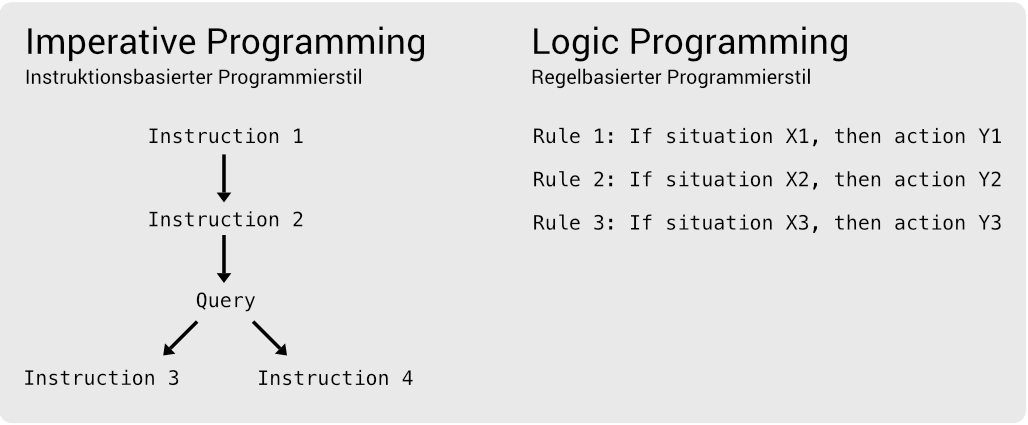
\includegraphics[width=17cm]{chapters/expertensysteme/imperative_vs_rule_based}
    \caption{Imperativer Programmierstil vs. Regelbasierter Programmierstil}
    \label{fig:programmierstil}
\end{figure}

\noindent So ein regelbasierter Ansatz hat vier wichtige Eigenschaften, die den einzelnen Komponenten des Systems zu Gute kommen. Eine Aneinanderreihung von WENN-DANN-Regeln ist\\

\begin{itemize}
    \item \textbf{Modular:} Das Wissen wird unabhängig voneinander in kleineren Regeln dargestellt.
    \item \textbf{Incrementable:} Aufgrund ihrer Modularität, können neue Regeln problemlos hinzugefügt werden.
    \item \textbf{Modifiable:} Das Ändern einer Regel beeinflusst nicht die restlichen Regeln.
    \item \textbf{Transparent:} Regeln können verwendet werden, um das Programmverhalten zu erklären.
\end{itemize}

%------------------------------- Aufbau eines Expertensystems --------------------------------
%---------------------------------------------------------------------------------------------
\subsection{Aufbau eines regelbasierten Expertensystems}
\noindent Regelbasierte Expertensysteme bestehen aus vier verschiedenen Komponenten:\\

\noindent {\fontfamily{pag}\selectfont {\small \textbf{Knowledge Base:}}}\\
Die Wissensbasis enthält das ganze Fachwissen der Experten.\\
Die ganzen WENN-DANN-Regeln sind hier gespeichert.\\

\noindent {\fontfamily{pag}\selectfont {\small \textbf{Inference Engine:}}}\\
Der Regelinterpreter bzw. der Logikkern des ganzen Systems. Mit Hilfe der Regeln aus der Knowledge Base, wird hier das Problem interpretiert, verarbeitet und gelöst.\\

\noindent {\fontfamily{pag}\selectfont {\small \textbf{Working Storage:}}}\\
Hier werden relevante Daten zur aktuellen Problemlösung zwischen gespeichert.\\

\noindent {\fontfamily{pag}\selectfont {\small \textbf{User Interface:}}}\\
Die Schnittstelle zwischen dem Benutzer und der Inference Engine.\\

\noindent Der Working Storage, die Benutzerschnittstelle sowie die Inference Engine bilden die Hülle des Systems. Die Knowledge Base soll theoretisch austauschbar sein, jedoch ist dies in der Praxis nur sehr schwer umsetzbar, denn die Inference Engine ist zu sehr auf das Wissen der Knowledge Base zugeschnitten.

\begin{figure}[H]
    \centering
    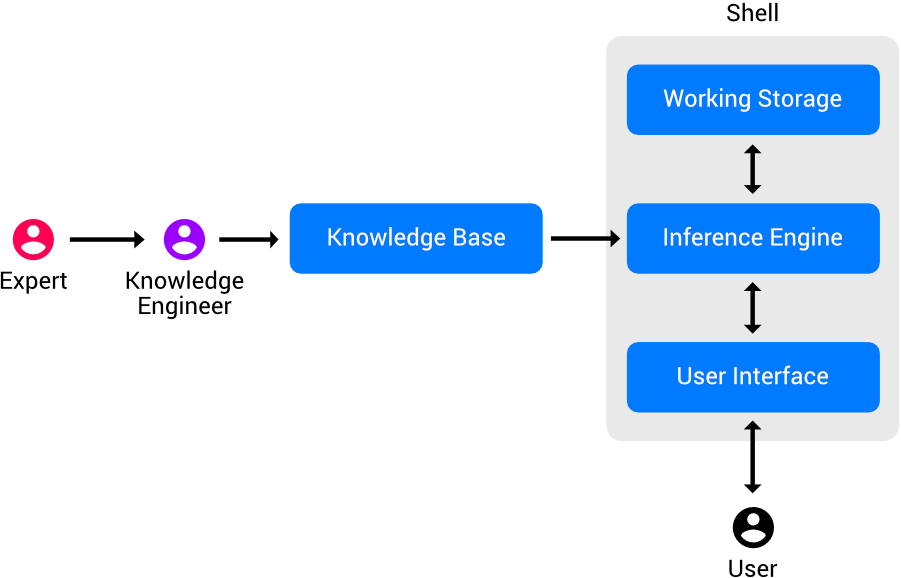
\includegraphics[width=17cm]{chapters/expertensysteme/aufbau_expertensystem}
    \caption{Aufbau eines regelbasierten Expertensystems}
    \label{fig:aufbau}
\end{figure}

%------------------------------- Wie wird Wissen abgearbeitet? --------------------------------
%----------------------------------------------------------------------------------------------
\subsection{Wie wird Wissen abgearbeitet?}
\noindent Die Inferenz der Regeln erfolgt intern über Goal Trees, auch AND-OR-Trees genannt. Ein Goal Tree weist die üblichen Baumeigenschaften auf. Das Topgoal ist die Wurzel des Baumes, dementsprechend sind die Subgoals die Teilbäume des Baumes, welche selbst wiederum Goal Trees sind. Es gibt zwei Arten von Knoten:\\

\noindent \textbf{AND-Knoten:} Hier müssen alle Teilbäume erfüllt werden.\\
\textbf{OR-Knoten:} Ein Teilbaum muss erfüllt werden.\\

\noindent Es gibt generell zwei verschiedene Ansätze um die Problemstellung zu lösen, entweder anhand des \textbf{Forward Chainings} oder seinem Gegenstück, anhand des \textbf{Backward Chainings}.



%----------------------------------------------------------------------------------------
%	Forward Chaining
%----------------------------------------------------------------------------------------
\section{Forward Chaining}
\noindent Das Forward Chaining wird auch \textbf{Data Driven Reasoning} genannt, denn man fängt mit einer gegebenen Faktenbasis \textit{(den Basiszuständen)} an. Dies sind die Blätter des Goal Trees. Von hier aus schließt man mit Hilfe der Regeln aus der Knowledge Base neue Fakten und tastet sich immer weiter vor bis man schlussendlich aus den geschlossenen Fakten eine Diagnose tätigen kann. Dies ist unser Topgoal, also die Wurzel des Goal Trees.\\

\noindent Zum Veranschaulichen ein kleines Beispiel aus der Tierwelt:\\
In der freien Natur sehen wir ein Tier, was wir identifizieren wollen. Um nun unser Problem zu lösen benutzen wir ein Expertensystem, welches mit der Methode des Forward Chaining arbeitet.
Wie oben bereits schon erwähnt fangen wir beim Forward Chaining mit einer Faktenbasis an. Auf unser Problem bezogen bedeutet dies, dass wir Beobachtungen aufstellen müssen. Zum Beispiel sehen wir, dass einige Tiere Federn haben, andere wiederum einen Schnabel. Einige leben in der Kälte, andere sind nachtaktiv. Mit Hilfe dieser Basiszustände versucht das System eine Lösung zu inferieren.\\

\begin{figure}[H]
    \centering
    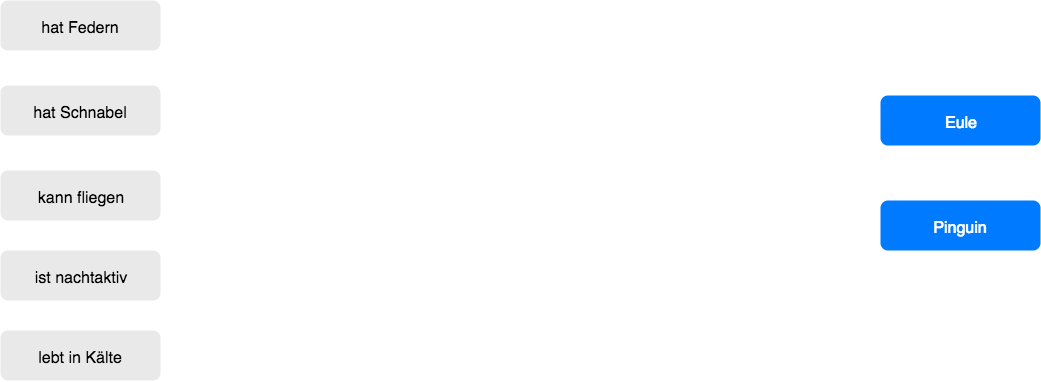
\includegraphics[width=17cm]{chapters/expertensysteme/forward_chaining/forward_chaining_1}
    \caption{Beginnen mit unserer Faktenbasis, hier links}
    \label{fig:forward_chaining_1}
\end{figure}

\noindent Mit den Regeln aus der Knowledge Base kann das System nun schrittweise zu Teillösungen voranschreiten. Die erste Regel könnte lauten: \textbf{WENN} Federn und \textbf{WENN} Schnabel, \textbf{DANN} Vogel.
\begin{figure}[H]
    \centering
    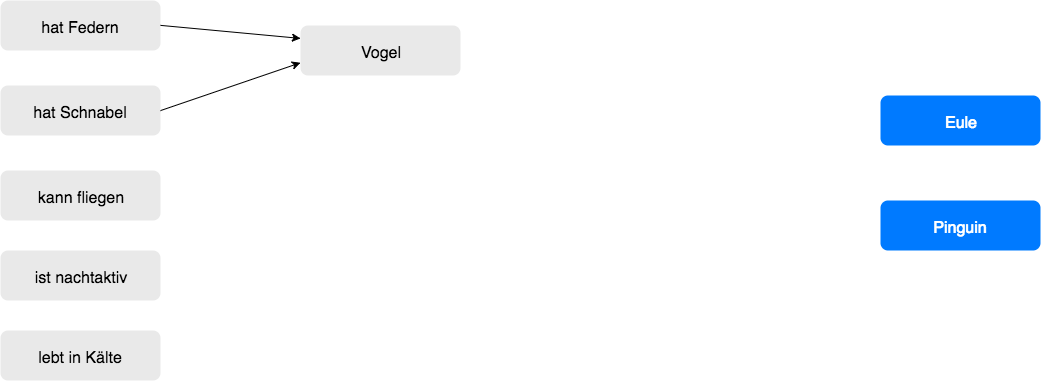
\includegraphics[width=17cm]{chapters/expertensysteme/forward_chaining/forward_chaining_2}
    \caption{Neue Teillösungen inferieren}
    \label{fig:forward_chaining_2}
\end{figure}

\noindent Eine andere Regel könnte lauten: \textbf{WENN} Vogel und \textbf{WENN} fliegen, \textbf{DANN} flugfähiger Vogel.
\begin{figure}[H]
    \centering
    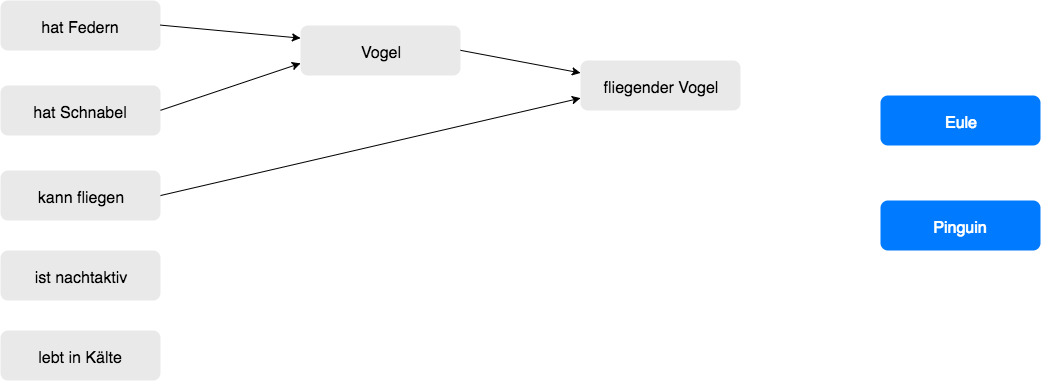
\includegraphics[width=17cm]{chapters/expertensysteme/forward_chaining/forward_chaining_3}
    \caption{Weitere Teillösung inferieren}
    \label{fig:forward_chaining_3}
\end{figure}

\clearpage
\noindent Eine weitere Regel könnte lauten: \textbf{WENN} fliegender Vogel und \textbf{WENN} nachtaktiv, \textbf{DANN} Eule. Somit hat unser Expertensystem von unseren anfänglichen Beobachtungen geschlussfolgert, dass es sich um eine Eule handeln muss.
\begin{figure}[H]
    \centering
    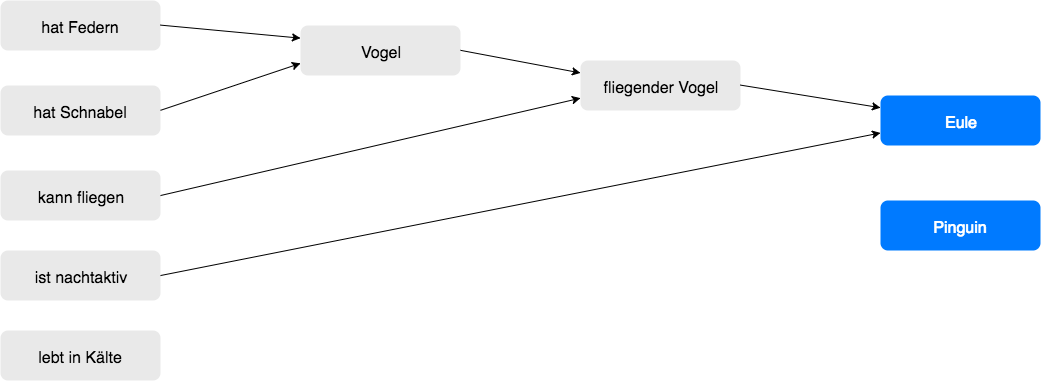
\includegraphics[width=17cm]{chapters/expertensysteme/forward_chaining/forward_chaining_4}
    \caption{Topgoal erreicht}
    \label{fig:forward_chaining_4}
\end{figure}

\noindent Würden wir nun ein weiteres Tier sehen und wieder unser Expertensystem fragen, könnte das ganze so aussehen:
\begin{figure}[H]
    \centering
    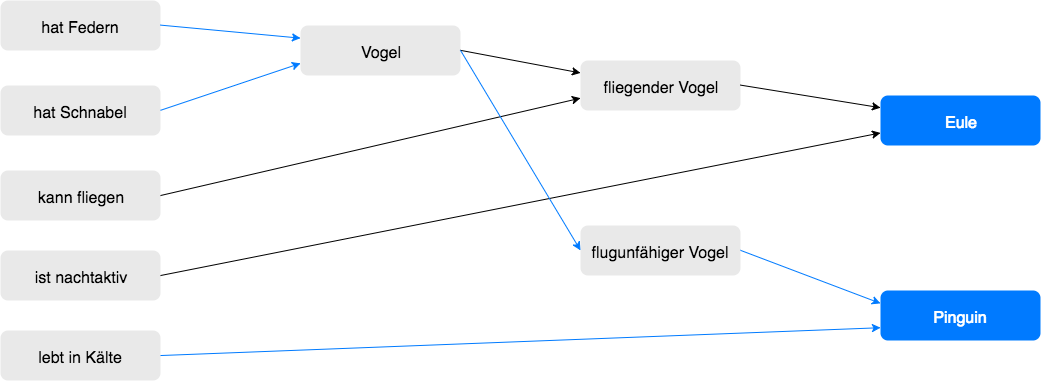
\includegraphics[width=17cm]{chapters/expertensysteme/forward_chaining/forward_chaining_5}
    \caption{Von unserer Faktenbasis inferiert das System, dass es sich um einen Pinguion handelt.}
    \label{fig:forward_chaining_5}
\end{figure}

\noindent Das Forward Chaining ist anwendbar auf Probleme mit nicht aufzählbaren Lösungen. In der Realität wird Forward Chaining daher in Design- und Konfigurationssysteme genutzt.



%----------------------------------------------------------------------------------------
%	Backward Chaining
%----------------------------------------------------------------------------------------
\section{Backward Chaining}
Backward Chaining ist wie vorher schon erwähnt das Gegenstück zum Forward Chaining. Hier beginnt man beim Topgoal und zerlegt dieses in die ursprünglichen Subgoals. Da die Subgoals prinzipiell wieder Topgoals sind zerlegt man diese auch wieder in Subgoal. Dies macht man solange bis man wieder bei den Blättern, also den Fakten angelangt ist. Man kann dazu auch sagen: Das System inferiert von den Hauptlösung zur Teillösung. Diese Teillösungen werden dabei im Working Storage gespeichert. Nun wird dies wieder an unserem bekannten Beispiel mit Eule und Pinguin illustriert.

\subsection*{Beispiel}
\begin{figure}[H]
    \centering
    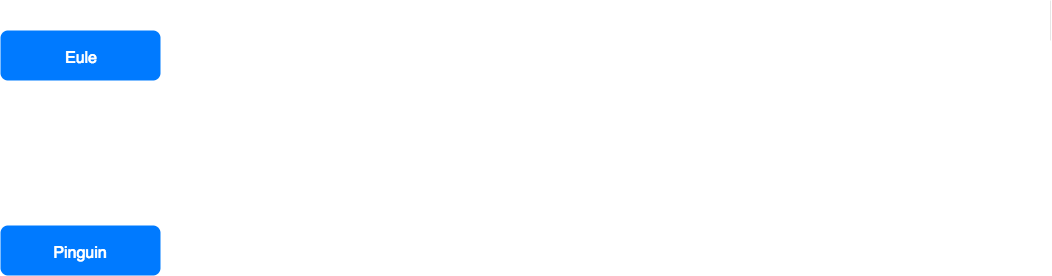
\includegraphics[width=17cm]{chapters/expertensysteme/backward_chaining/backward_chaining_1}
    \label{fig:backward_chaining_1}
\end{figure}

Wir haben nun die beiden Topgoals Eule und Pinguin gegeben. Nun möchten wir wieder zu den Teillösungen gelangen. Dies geschieht wie auch beim Forward Chaining mit den Wenn-Dann Regeln. In diesem Beispiel wäre die erste Regel:

Wenn Eule, dann kann fliegen und ist nachtaktiv

\begin{figure}[H]
    \centering
    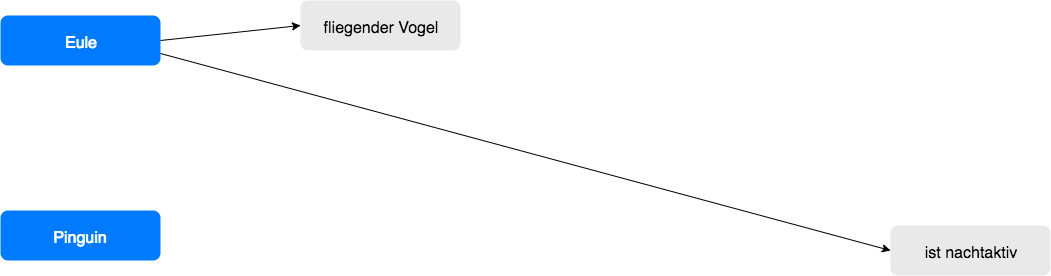
\includegraphics[width=17cm]{chapters/expertensysteme/backward_chaining/backward_chaining_2}
    \label{fig:backward_chaining_2}
\end{figure}

Dies macht man nun solange bis man wieder bei der Faktenbasis ist.

\begin{figure}[H]
    \centering
    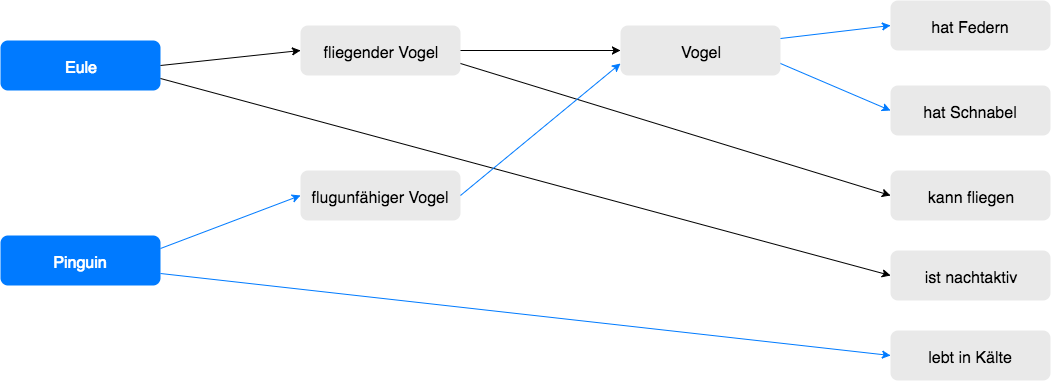
\includegraphics[width=17cm]{chapters/expertensysteme/backward_chaining/backward_chaining_3}
    \label{fig:backward_chaining_3}
\end{figure}

\noindent Diese Art von regelbasierten Expertensystem ist anwendbar auf Probleme mit strukturierter Selektion und auf Probleme, die aufzählbare Lösungen haben. Hier könnte sich die Frage stellen: Warum nur auf Probleme mit aufzählbaren Lösungen? Diese Frage beantwortet sich fast schon von allein, da jede Lösung mindestens eine Regel haben muss.

\noindent In der Realität wird Backward Chaining daher in Identifaktions- und Diagnosesysteme zum Einsatz.


%----------------------------------------------------------------------------------------
%	Umgang mit Unsicherheit
%----------------------------------------------------------------------------------------
\section{Umgang mit Unsicherheit}
Im regelbasierten Expertensystem gibt es nur absolute Angaben, also nur richtig oder falsch. Dies ist aber nicht Realitätsnah, da Benutzer nicht immer absolut sicher sind. Außerdem kann es auch sehr gut sein, dass Unsicherheiten in den Regeln vorkommen. Durch all diese Unsicherheiten gibt es das Bedürfnis mit diesen Unsicherheiten umzugehen. 

Eine Möglichkeit mit den Unsicherheiten sind die Certainty Factors (CF) zu deutsch Sicherheitsfaktoren.

\subsection{Certainty Factors}
Die CF's liegen zwischen -1 und 1. Dabei entspricht -1 falsch, 1 wahr und 0 kompletter Unwissenheit. Den CF des Topgoals kann man berechnen, in dem man den minimalen CF der Subgoals mit dem CF der abschließenden Regel multipliziert. Dies wird im nächsten Beispiel veranschaulicht. Desweiteren gilt:
\begin{itemize}
	\item ist ein Subgoal mit -1 bewertet, so ist das Topgoal nicht erfüllbar
	\item erhält das Topgoal einen CF mit 1, so ist dieses mit Sicherheit erfüllbar.
\end{itemize}
In manchen Systemen kann es vorkommen, dass die Werte -1 und 1 als sehr mächtig interpretiert werden und man noch andere Werte zu lassen möchte. Daher kann man sich eigene Schwellen einrichten, so könnte man Beispielsweise sagen: "`Wir erkennen schon einen Wert ab 0.75 als wahr an und einen -0.75 als falsch."' Aber auch dies ist immer System und Benutzer abhängig. 

\subsection*{Beispiel}
Betrachten wir nun die Regel:

{\bfseries Wenn flugunfähiger Vogel und lebt in Kälte dann Pinguin.}

\begin{itemize}
\item {\bfseries flugunfähiger Vogel} ist ein Subgoal welches durch alle Regeln und Subgoals, die zu ihm führen mit einem CF=0.4 bewertet wurde.
\item {\bfseries lebt in Kälte} ist ein Fakt, welcher einen CF=-0.3 erhalten hat. Dieser wurde vom Benutzer eingegeben. 
\item Die {\bfseries Wenn-Dann-Regel} ist eine sehr sichere Regel die mit 0.9 bewertet wurde. Man könnte sich noch vorstellen, dass der flugunfähige Vogel in der Kälte eine Möwe mit gebrochenen Flügel ist, aber das ist auch schon alles.
\end{itemize}

Der minimale Wert der Subgoals ist hier -0.3.

$\Rightarrow$ CF für Pinguin $-0.3 \cdot 0.9 = -0.27$

Die -0.27 sagen uns nun das wir eher nicht wissen, dass es ein Pinguin ist, aber wir schon sehr unsicher sind ob es wirklich kein Pinguin ist.



Es kann vorkommen, dass es in einem regelbasierten Expertensystem mehrere Wege gibt, um auf das gleiche Ziel zu gelangen. Wenn dieser Fall eintritt möchte man die CF's, die durch die verschiedenen Regeln für das gleiche Topgoal entstehen in irgendeiner Form kombinieren können. Dazu gibt es verschiedene Möglichkeiten. Eine dieser Möglichkeiten ist unter anderem MYCINs Certainty Algebra.


\subsection{MYCINs Certainty Algebra}
Als Voraussetzung für diese Algebra muss man mindestens $2$ CF's haben, die man kombinieren möchte, also X und Y. 
Hat man dies gegeben, so kann man den kombinierten CF mit Hilfe der folgenden Algebra berechnen:

	$$
	CF(X,Y) = 
	\begin{cases}
		X+Y \left(1-X\right) 
		  & X \ge 0 \wedge Y \ge 0 \\
		\left( X+Y\right)
		/ \left(1-min \left(|X|, |Y|\right)\right) &  X < 0 \vee Y < 0 \\
		X+Y \left(1+X\right)  & X < 0 \wedge Y < 0
	\end{cases}
	$$

Wenn man mehr als 2 CF's gegeben hat, dann kombiniert man 2 und das Ergebnis dann mit den weiteren 

z.B.: a, b, c kombiniere erst d=CF(b,c) erg=CF(a,d)

$\Rightarrow$ Die Reihenfolge spielt hier also keine Rolle.



\subsection*{Beispiel zur Kombination von CF's mithilfe von MYCINs Certainty Algebra}
Regeln:
\begin{itemize}
		\item[1.] flugunfähiger Vogel, isst Fisch, lebt auch in der Antarktis $\Rightarrow$ Pinguin CF=0.51
		\item[2.] flugunfähiger Vogel, ist schwarz/weiß, kann schwimmen $\Rightarrow$ Pinguin CF=-0.3
			\item[3.]  Vogel, isst Fisch, kann schwimmen, lebt auch in der Antarktis $\Rightarrow$ Pinguin CF=0.4
\end{itemize} 
Nun haben wir den Fall, dass wir 3 Regeln haben, die man kombinieren möchte.
Zuerst sei X=0.51 und Y=-0.3, also haben wir den Fall, dass einer der Werte unter 0 ist und der andere über 0. Daher müssen wir $CF \left( X,Y \right) =\left( X+Y\right) / \left(1-min \left(|X|, |Y|\right) \right)$ anwenden. Also:


$CF \left( 0.51,-0.3 \right) =\left( 0.51-0.3 \right) / \left(1-min \left(|0.51|, |-0.3|\right) \right)$ \\
Das ergibt 0.3. 
Nun muss noch die 0.3 mit der 0.4 kombiniert werden. Wenn man dies macht kommt ein Wert von 0.58.



%----------------------------------------------------------------------------------------
%	Verhalten erklören
%----------------------------------------------------------------------------------------
\section{Verhalten erklären}
\noindent Expertensysteme können ihr Verhalten dem Nutzer erklären, sollte dieser eine simple Nachfrage stellen. Hierbei wird zwischen zwei Arten von Fragen unterschieden.

\subsection{Why-Questions}
\noindent Why-Questions sind Fragen die angeben, warum die genau diese Anfrage dem Nutzer gestellt wurde. In einem Goal Tree muss sich das System nur eine Ebene nach oben bewegen um die Antwort auf die gestellte Frage zu finden.\\

\noindent {\fontfamily{pag}\selectfont {\small \textbf{Beispielaufruf:}}}\\
\noindent \textbf{System:} Ist fliegender Vogel?\\
\textbf{User:} why?\\
\textbf{System:} Eule $\Leftarrow$ fliegender Vogel, ist nachtaktiv

\subsection{How-Questions}
\noindent How-Questions beantworten warum diese spezifische Lösung inferiert wurde. Das Expertensystem hat sich seinen Arbeitsweg abgespeichert und ruft diesen Schritt für Schritt ab, falls der Nutzer Fragen stellt.\\

\noindent {\fontfamily{pag}\selectfont {\small \textbf{Beispielaufruf:}}}\\
\noindent \textbf{System:} Tier ist Eule.\\
\textbf{User:} how Eule?\\
\textbf{System:} fliegender Vogel, ist nachtaktiv $\Rightarrow$ Eule\\
\textbf{User:} how fliegender Vogel?\\
\textbf{System:} Vogel, kann fliegen $\Rightarrow$ fliegender Vogel


%----------------------------------------------------------------------------------------
%	Zusammenfassung
%----------------------------------------------------------------------------------------
\section{Zusammenfassung}
Expertensysteme simulieren menschliche Experten, die nur aus WENN-DANN-Regeln bestehen. Die Lösungen, die die Expertensysteme generieren sind basiert auf Regeln, die von der Problemstellung vorgegeben werden. Es kann mit Unsicherheiten umgehen, sei es Unsicherheiten in den Regeln oder auch von der Benutzereingabe her. Das Programm kann sich selbst erklären solange die Fragen How bzw. Why basiert sind.

\begin{table}[H]
    \centering
    \label{zsmfassung_Chaining}
    \begin{tabular}{c|c|c}
                                    &\textbf{Forward Chaining}                  &\textbf{Backward Chaining}         \\\hline
        \textbf{Ansatz}             & Data Driven Reasoning                     & Goal Driven Reasoning             \\\hline
        \textbf{Goal Tree}          & von Blättern aufgebaut                    & von Wurzel aufgebaut              \\\hline
        \textbf{Lösungen finden}    & Lösungszustände durch Regeln akzeptiert   & Jede Lösung (mind.) ein Topgoal   \\\hline
        \textbf{Anwendung}          & nicht aufzählbare Lösungsmenge            & aufzählbare Lösungsmenge          \\
    \end{tabular}
\end{table}



%----------------------------------------------------------------------------------------
%	Kritikpunkte
%----------------------------------------------------------------------------------------
\section{Kritikpunkte}
Es gibt einige Kritikpunkte an den Expertensystemen, da die Knowledge Base aufwändig zu erstelle ist. Meistens benötigt man einen Experten und zustätzlich noch einen Knowledge Engineer, der das Expertenwissen in eine regelbasierte Computersprache umsetzen kann. Das Wissen des Expertensystems ist kein echtes Wissen, sondern nur regelbasiert, somit kann nur neues Wissen angelegt werden, wenn dieses wieder in die Regelform gebracht wurde. Es gibt zwar die Möglichkeit das System zu hinterfragen mit den How- und Why-Questions, jedoch gibt das System meistens nur die Position im Goal Tree an, aber kein Hintergrundwissen oder Begründungen für den Benutzer.
\input{chapters/theoremprovers/tp}
\chapterimage{chapter_head_1.png}

\chapter{Bayessche Netze}

\section{Intro}
Ein Bayessches Netz stellt die Wahrscheinlichkeiten von Ereignissen und deren Abhängigkeit (bzw. Unabhängigkeit) zueinander dar.

Bayessche Netze finden immer dort Anwendungsmöglichkeit, wo Logik und Unwissenheit aufeinandertreffen.
Sie dienen der Vereinfachung von komplexen Problemen mit Hilfe weniger stochastischer Regeln.

In der Praxis finden Bayessche Netze beispielsweise in der Spracherkennung, medizinischen Diagnose, Filtern von Spam, Bildverarbeitung, Analyse von Kaufverhalten und in vielen anderen Gebieten Anwendung.

\begin{figure}[h]
    \centering
    \includegraphics[width=.4\textwidth]{chapters/bayes/bayes_intro.pdf}
    \caption{Beispiel eines Bayesschen Netzes zur Diagnose von Krankheiten (ohne Wahrscheinlichkeiten)}
\end{figure}

\section{Grundlagen der Wahrscheinlichkeitsrechnung}
Einem Ereignis A weisen wir eine Wahrscheinlichkeit p(A) zwischen 0 (tritt nie ein) und 1 (tritt immer ein) zu.

Als marginal probability bezeichnen wir eine Wahrscheinlichkeit p(A), welche keine Abhängigkeiten aufweist.
Beispiel: A = Eine aus einem Skatdeck gezogene Karte ist Kreuz.
p(A) = 1/4 (oder 25~\%)

Als joint probability bezeichnen wir Wahrscheinlichkeiten, welche nebeneinander auftreten. p(A,B)
Beispiel: A (von oben) und B: Die Karte ist ein Bube

Da A und B voneinander unabhängige Ereignisse sind folgt:
p(A,B) = p(A) $\cdot$ p(B) = 1/8 $\cdot$ 1/4 = 1/32

Sind Ereignisse jedoch nicht unabhängig, so müssen wir die Wahrscheinlichkeit von p(A,B) bereits bestimmt haben.
Möchten wir nun für eine große Anzahl Ereignisse Wahrscheinlichkeiten berechnen, so benötigen wir extrem viele Daten.

\begin{center}
\begin{tabular}{ ccccc } \toprule
Sonne scheint & Werktag & Stau & Rasensprinkler & Tage im Jahr \\ \midrule
F & F & F & F & 4 \\
F & F & F & T & 5 \\
F & F & T & F & 2 \\
F & F & T & T & 1 \\
F & T & F & F & 13 \\
F & T & F & T & 2 \\
F & T & T & F & 66 \\
F & T & T & T & ... \\
T & F & F & F & ... \\
T & F & F & T & \\
T & F & T & F & \\
T & F & T & T & \\
T & T & F & F & \\
T & T & F & T & \\
T & T & T & F & \\
T & T & T & T & Errechenbar \\
\bottomrule
\end{tabular}
\end{center}


Bis auf 1 errechenbares Ergebnis benötigen wir die direkten Werte aller Kombinationen.
Wir benötigen also Für N Ereignisse $2^N-1$ Datensätze.
Gerade in der Medizin aus dem Anfangsbeispiel gibt es aber oft extrem viele Ereignisse.

Oftmals ist vieles davon aber auch nicht interessant, bzw. ableitbar.
Die Wahrscheinlichkeit, dass die Sonne scheint ist beispielsweise unabhängig davon ob der Tag ein Werktag ist.

Um die benötigten Datensätze möglichst gering zu halten betrachtet man bedingte Wahrscheinlichkeiten (conditional probability).

\section{Bedingte Wahrscheinlichkeit}
Bedingte Wahrscheinlichkeiten beruhen auf Annahmen.
Man nimmt etwa an, dass die Sonne keinen Einfluss auf die Frage hat, ob es nun ein Werktag ist, sehr wohl jedoch auf die Frage, ob der Sprinkler angeschaltet ist.
Gehen wir weiterhin davon aus, dass an sonnigen Tagen mehr Staus zustande kommen, da z.B. Fahrer geblendet werden.
Zudem gehen wir davon aus, dass werktags mehr Staus auftreten.
Fügen wir zudem noch das Verpassen des Essens hinzu, welches lediglich vom Stau abhängt.

\begin{figure}[h]
    \centering
    \includegraphics[width=.2\textwidth]{chapters/bayes/bayes_example.pdf}
\end{figure}

Unsere benötigten Datensätze mit fiktivem Inhalt:\\
$p(Sonne) = 0,8$\\
$p(Werktag)= 0,7$\\
$p(Rasensprinkler | Sonne) = 0,95$\\
$p(Rasensprinkler | !Sonne) = 0,20$\\
$p(Stau | Sonne,Werktag) = 0,8$\\
$p(Stau | !Sonne, Werktag) = 0,75$\\
$p(Stau | Sonne, !Werktag) = 0,15$\\
$p(Stau | !Sonne, !Werktag) = 0,05$\\
$p(Essen verpasst | Stau) = 0,5$\\
$p(Essen verpasst | !Stau) = 0,05$\\

Von 31 Datensätzen in einer Tabelle mit joint probabilities haben wir nun nur noch 10 benötigt Wahrscheinlichkeiten und können alle anderen nun problemlos errechnen. (Beispiel folgt)

Um bedingte Wahrscheinlichkeiten effektiv nutzen zu können benötigen wir einige Definitionen:
\begin{equation*}
p(A,B) = p (A | B) \cdot p (B)
\end{equation*}
Daraus folgt direkt:
\begin{equation*}
p(A,B,C) = p(A | B,C) \cdot p(B,C) = p(A | B,C) \cdot p(B | C) \cdot p(C)
\end{equation*}
Dies lässt sich für N Ereignisse wie folgt darstellen (Chain Rule):
\begin{equation*}
P\left(\bigcap_{k=1}^N A_k\right)  = \prod_{k=1}^N  \mathrm P\left(A_k \,\Bigg|\, \bigcap_{j=1}^{k-1} A_j\right)
\end{equation*}
Zudem bezeichnen wir A als von B unabhängig, wenn gilt:
\begin{equation*}
p(A | B) = p(A)
\end{equation*}
und A als von B unabhängig unter der Prämisse C, wenn gilt:
\begin{equation*}
p(A | C) \cdot p(B | C) = p(A,B | C)
\end{equation*}
%
Mit Hilfe der Chain-Rule können wir nun für das Beispiel von oben jede mögliche joint probability ausrechnen.
%
\subsection{Rechenbeispiel}
Wir suchen eine Möglichkeit folgenden Ausdruck zu berechnen:
\begin{equation*}
p(Essen ~verpasst,Stau,Werktag,Rasensprenger,Sonne)
\end{equation*}
Nach Anwendung der Chain Rule haben wir:
\begin{align*}
& p( Essen ~verpasst | Stau , Werktag, Essen ~verpasst, Sonne )\\
\cdot & p( Stau | Werktag , Rasensprinkler, Sonne )\\
\cdot & p( Werktag | Rasensprinkler, Sonne )\\
\cdot & p( Rasensprinkler | Sonne )\\
\cdot & p( Sonne )
\end{align*}
Wichtig ist hier den Aufbau des ersten Ausdrucks entlang der Abhängigkeiten zu formulieren. Die Reihenfolge der Ereignisse für die joint probabilty muss also eine umgedrehte topologische Anordnung unseres Graphen darstellen bzw. ein Ereignis A kann nicht vor einem Ereignis B stehen, wenn B abhängig von A ist.\\
Nach dem Kürzen der Unabhängigkeiten erhalten wir:
\begin{align*}
p(Essen ~verpasst | Stau ) 
\cdotp( Stau | Werktag, Sonne)
\cdot p(Werktag) 
\cdot p(Rasensprinkler | Sonne)
\cdot p(Sonne)
\end{align*}
Man nennt dies auch die Faktorisierung.\\
Die gesuchten Wahrscheinlichkeiten kennen wir bereits und können sie einsetzen:
\begin{equation*}
0,5 \cdot 0,8 \cdot 0,7 \cdot 0,95 \cdot 0,8 = 0,218.
\end{equation*}
%
Es ist also durch simples Einsetzen unserer 10 Werte möglich sämtliche 31 Werte für die joint probability Tabelle zu berechnen.
Gleichzeitig sind Lösungen für relevante Fragen zur bedingten Wahrscheinlichkeit, welche nicht alle Ereignisse umfassen, mit geringem Aufwand zu lösen.
%
In der Regel sind jedoch nicht alle Angaben bekannt.
Nehmen wir nun an, dass wir als hart arbeitender Mensch an einem Nicht-Werktag zur Arbeit fahren und es sonnig ist.
Wir möchten nun wissen, wie wahrscheinlich es ist, dass man es abends bei der Rückfahrt rechtzeitig zum Essen schafft.
Wir suchen also:
\begin{equation*}
p(!Essen ~verpasst | !Werktag, Sonne)
\end{equation*}
Dazu berechnen wir:\\
\begin{equation*}
p(\!Essen ~verpasst | Stau) \cdot p(Stau | Sonne, \!Werktag) + p(\!Essen ~verpasst | \!Stau)
\cdot p(\!Stau | Sonne, \!Werktag)
\end{equation*}
%
Die passenden Werte kennen wir entweder oder können sie direkt ableiten:
\begin{align*}
&p(Essen ~verpasst | Stau) = 0,5 \rightarrow p(\!Essen ~verpasst | Stau) = 0.5\\
&p(Essen ~verpasst | \!Stau) = 0,05 \rightarrow p(\!Essen ~verpasst | \!Stau) = 0.95\\
&p(Stau | Sonne, \!Werktag) = 0,15 \rightarrow p(\!Stau | Sonne, \!Werktag) = 0.85\\\\
&0,5 \cdot 0,15 + 0,95 \cdot 0,85 = 0,8825 
\end{align*}
%
bzw. die Wahrscheinlichkeit am Wochenende pünktlich zum Essen zu kommen beträgt 88\%.\\
Was jedoch, wenn ich in die andere Richtung rechnen möchte?
Beispiel: Der Lebensgefährte kommt pünktlich zum Essen und ich möchte wissen, wie wahrscheinlich es ist, dass er im Stau gesteckt hat.
%
Wir kennen bereits die Formel:
\begin{equation*}
p(A,B) = p (A | B) \cdot p(B)
\end{equation*}
offensichtlich gilt auch:
\begin{align*}
&p(B,A) = p (B | A) \cdot p(A) \\
\Rightarrow & p(A | B) = p(A,B) / P(B) = p(B,A) / P(B) = p(B | A) \cdot p(A)/p(B) ~\text{(Satz von Bayes)}
\end{align*}
%
Wir wissen also:
\begin{align*}
&p(Stau | !Essen ~verpasst) = p(!Essen ~verpasst | Stau ) *P(Stau)/p(! Essen ~verpasst)\\
&p(!Essen ~verpasst | Stau) =0,5\\
p(Stau) =&p(Stau | Sonne, Werktag) \cdot p(Sonne) \cdot p(Werktag) + \\
&p(Stau | Sonne, !Werktag) \cdot p(Sonne) \cdot p(!Werktag)+ \\
&p(Stau | !Sonne, Werktag) \cdot p(!Sonne) \cdot p(Werktag) + \\
&p(Stau | !Sonne, !Werktag) \cdot p(!Sonne) \cdot p(!Werktag)= 0,382\\
&p(!Essen ~verpasst) =\\
&p(!Essen ~verpasst | Stau) \cdot p(Stau) + p(!Essen ~verpasst | !Stau) \cdot p(!Stau) = 0,7781 \\
&\Rightarrow p(Stau | !Essen ~verpasst)=0,5 \cdot 0,382/0,7781 = 0,2454...
\end{align*}
%
Ist die Person also pünktlich, so gab es mit einer Wahrscheinlichkeit von ~75\% keinen Stau.
%
An dieser Stelle ist anzufügen, dass das ganze Problem auch so hätte modelliert werden können, dass die Pünktlichkeit beim Essen ebenfalls vom Werktag abhängig ist, dann jedoch wäre die Abhängigkeit zum Stau zu hinterfragen, wenn es denn keinen Werktag gibt.
Es gibt also durchaus komplexere Problemstellungen, die wir mit unseren einfachen Methoden nicht so einfach behandeln können und eventuell verschiedene Modelle für Abhängigkeiten die je nach der Menge der Daten möglicherweise nicht optimal sind.
%
Diese neue Methode hilft uns vor allen Dingen damit mit einem einzelnen Modell gleichzeitig z.B. Krankheiten und Symptome in beide Richtungen zu bestimmen. Ohne große Umstände kann eine Krankheit aus Symptomen bestimmt werden und direkt von der Wahrscheinlichkeit der Krankheit kann die Wahrscheinlichkeit für weitere Symptome berechnet werden.
%
\section{Graphische Darstellung}
\begin{figure}[h]
    \centering
    \includegraphics[width=.2\textwidth]{chapters/bayes/bayes_net_1.pdf}
\end{figure}
\begin{figure}[h]
    \centering
    \includegraphics[width=.2\textwidth]{chapters/bayes/bayes_net_2.pdf}
\end{figure}
\begin{figure}[h]
    \centering
    \includegraphics[width=.2\textwidth]{chapters/bayes/bayes_net_3.pdf}
\end{figure}
\begin{figure}[h]
    \centering
    \includegraphics[width=.2\textwidth]{chapters/bayes/bayes_net_4.pdf}
\end{figure}

Wir nennen zwei Ereignisse X und Y bedingt unabhängig gegeben E, wenn im Graphen kein Weg von X zu Y existiert, welcher nicht E nicht beinhaltet.
Dies wir auch d-Separation genannt.
Wir schreiben hierfür
$X \perp Y | E$
Ausgehend vom vorherigen Beispiel heißt das, dass das Verpassen des Essens zwar vom Werktag abhängt, jedoch wenn bekannt ist, ob es einen Stau gab, diese Abhängigkeit aufgehoben wird.
Für 3 verknüpfte Ereignisse gibt es die Folgenden Möglichkeiten:
\begin{enumerate}[label=(\alph*)]
\item $A \rightarrow B \rightarrow C$ impliziert $A \perp C | B$
\item $A \leftarrow B \leftarrow C$ impliziert $A \perp C | B$
\item $A \leftarrow B \rightarrow C$ impliziert $A \perp C | B$
\item $A \rightarrow B \leftarrow C$ impliziert $A \perp C$
\end{enumerate}
Das Beispiel (d) beschreibt hierbei eine sogenannte V-Struktur.

Betrachten wir hierzu außerdem die Verschiedenen Faktorisierungen:
\begin{enumerate}[label=(\alph*)]
\item p(A,B,C) = p(C|B) $\cdot$ p(B|A) $\cdot$ p(A)
\item p(A,B,C) = p(A|B) $\cdot$ p(B|C) $\cdot$ p(C)
\item p(A,B,C) = p(A|B) $\cdot$ p(C|B) $\cdot$ p(B)
\item p(A,B,C) = p(B|A,C) $\cdot$ p(A) $\cdot$ p(C)
\end{enumerate}

\section{IC-Algorithmus}
Der IC Algorithmus ist eine Möglichkeit aus gegebenen Unabhängigkeiten ein Bayessches Netz zu erstellen.
\begin{enumerate}
\item Konstruiere einen ungerichteten Graphen; füge jede mögliche Kante (X,Y), für die es keine (bedingte) Abhängigkeit $X \perp Y | E$ bzw. $X \perp Y$ gibt, in den Graphen ein.
\item Gilt für zwei Nachbarn X,Y von einem Knoten E die bedingte Unabhängigkeit $X \perp Y | E$ nicht, dann füge die Kanten (X,E) und (Y,E) hinzu. (V-Struktur)
\item Orientiere die verbleibenden Kanten beliebig, aber ohne neue V-Strukturen entstehen zu lassen.
\end{enumerate}

\section{Erstellung eines Bayesschen Netzes}
Nach unseren theoretischen Überlegungen sind wir zur Erkenntnis gelangt, dass uns Bayessche Netze nicht nur ein intuitives Verständnis bzgl.
bedingten Wahrscheinlichkeiten vermitteln, indem Abhängigkeitsverhältnisse zwischen Zufallsvariablen explizit angegeben werden, sondern
auch langwierige Rechnungen erheblich vereinfachen können. Allerdings stellt sich für uns immer noch die Frage, wie wir aus einem
probabilistischen Problem ein geeignetes Netz entwickeln können.


\subsection{Aufbau eines Bayesschen Netzes aus Expertenwissen}   
Eine Möglichkeit wäre die Hilfe von Experten in Anspruch zu nehmen. Ihre Aufgabe besteht darin Abhängigkeitsverhältnisse anzugeben und
somit eine Topologie zu entwickeln sowie die entsprechenden Parameter der Knoten anzupassen. Diese Herangehensweise ist jedoch meist
nur für kleine bzw. unveränderliche Probleme geeignet, da sie zahlreiche Schwierigkeiten mit sich bringt.
Zum einen existiert ein Komplexitätsproblem. Offensichtlich kann allein die schiere Anzahl von Zufallsvariablen diesen Lösungsversuch
zunichtemachen. Aber wie ist es mit einer begrenzten, übersichtlichen Anzahl an Zufallsvariablen? 

Erinnern wir uns an die Kanten des Graphen. Jede Kante beschreibt eine Wahrscheinlichkeit und  kann einen Wert zwischen 0 und 1 annehmen.
Somit ist jede Wahrscheinlichkeit maximal eine gute Approximation der Realität. Da es oft der Fall ist, dass jede Zufallsvariable von
mehreren Eltern abhängt und ihrerseits die Wahrscheinlichkeit ihrer Kinder bestimmt, können bereits kleinste Fehler zu großem Schaden
führen und das Bayes Netz somit unbrauchbar machen. 
Dies lässt die Schlussfolgerung zu, dass ein konstruiertes Netz von verschiedenen Experten auf Fehler untersucht werden sollte, sodass
der ganze Entwicklungsprozess sehr langwierig wird. Dennoch kann das Ergebnis nicht verifiziert werden.

\subsection{Aufbau eines Bayesschen Netzes aus selbstlernenden Algorithmen} 
Da der Aufbau eines Bayesschen Netzes aus Expertenwissen einige Probleme mit sich bringt, haben Wissenschaftler eine weitere Methode
entwickelt. Sie besteht darin, dass Netz in die Lage zu versetzen, anfallende Daten zu analysieren und auf Grundlage des Ergebnis
Justierungen vorzunehmen. Da solche Algorithmen sehr komplex sind, werden im folgenden nur die Grundzüge der Verfahren vorgestellt
und einhergehende Schlüsselwörter genannt. Grundsätzlich gibt es zwei Möglichkeiten ein Netz zu erstellen bzw. zu verbessern.

\subsubsection{Anpassung der Parameter}
Ein Experte erstellt eine sinnvolle Topologie und fügt Parameter ein. Diese Parameter beruhen auf A-priori Wahrscheinlichkeiten und 
sollten eine gute Approximation darstellen. Solch ein Netz wird „augmented Bayesian network“ genannt. Die Idee besteht darin,
dass die Werte der Parameter kontinuierlich an die anfallenden Daten angepasst werden. Dies hat zur Folge, dass dasNetz umso bessere
Vorhersagen treffen kann, je mehr Daten bereits verarbeitet wurden. In diesem Kontext spielt besonders dierelative Häufigkeit
eine wichtige Rolle. Darunter versteht man wie oft ein gewisses Ereignis in einer Zeitspanne eintrat.\\
Beispiel: Wir werfen eine Münze. Wir schätzen, dass die Wahrscheinlichkeit 50 \% beträgt, dass das Ereignis Kopf eintritt. Nach dem 
10.000 Wurf stellen wir fest, dass 7000 mal das Ereignis Kopf eingetreten ist. Somit beträgt die relative Häufigkeit 70 \% und wir
müssen unseren anfangs gewählten Wert anpassen. \\
Diese Art von Berechnung ist jedoch nur möglich, wenn die relative Häufigkeit eines Parameters mit  [0,1] gleich wahrscheinlich ist. 
In vielen Fällen muss jedoch ein anderer Weg eingeschlagen werden, da diese Art von Verteilung nicht angenommen werden kann. Somit
benötigen wir eine Verteilungsfunktion, die in der Lage ist solche Verteilungen darzustellen.
Zu diesem Zweck bietet sich besonders die Familie der Beta Wahrscheinlichkeitsdichtefunktionen an, da diese über die Eigenschaft
verfügen, nach Dateneingang dynamisch und kontinuierlich angepasst werden zu können. 

\subsubsection{Erstellung der Topologie}
Die zweite Möglichkeit ein Bayes Netz durch Algorithmen konfigurieren zu lassen, besteht darin die Struktur eines Bayesschen
Netzes entsprechend der Datenlage anzupassen.
Eine populäre Methode ist der „score-based approach“. Dabei wird jeder Struktur ein Score zugewiesen, der angeben soll, wie geeignet
gegebene Daten durch eine beliebige Struktur beschrieben werden. Der Score wird folgendermaßen berechnet:\\
\\
P(G|D) = Score(G, D),
mithilfe der Bayesschen Formel zu

\begin{equation}
 P(G|D) = \frac{{P(D|G) * P(G)}}{{P(D)}}
\end{equation}

Da uns die zur Verfügung gestellten Daten nicht weiter interessieren, konzentrieren wir uns einzig auf den Zähler, da wir das Ziel
haben diesen Ausdruck zu maximieren.
P(G) kann durch verschiedene Möglichkeiten mithilfe von „prior information“ bestimmt werden.
Prior information geben Wahrscheinlichkeitsverteilungen an,  bevor es Beweise für deren Richtigkeit gibt. Sie beruhen meist auf
früheren Beobachtungen oder entstehen durch Vergleich mit ähnlichen Problemen.
Somit liegt der Fokus in der Maximierung von P(D|G). Es wurden viele verschiedene Möglichkeiten entwickelt dieses Problem zu
lösen, eine Standardmethode beinhaltet meistens die Likelihood-Berechnung, ein Schätzverfahren, dass die Maximierung eines
Ausdrucks anstrebt durch  Schätzen der Parameter anstrebt. 



\subsection{Vorteile von Bayesschen Netzen}			
Bayessche Netze ersparen ihren Anwender enorm viel Arbeit. Sie reduzieren die benötigten Wahrscheinlichkeitstabellen auf ein Minimum,
sodass manche Anwendungen laufzeit-technisch erst möglich werden.
Beispielsweise benötigt die Berechnung der Joint probability eine Laufzeit aus O($2^{n}$), unter der Bedingung, dass die gewählten
Zufallsvariablen binär sind, mithilfe von unserem Netz eine Laufzeit aus O($2^{pa(x)}$) wobei pa(x) für die Anzahl aller Eltern eines
Knotens x steht. 

Ein weiterer Vorteil von einem Bayes Netz liegt darin, dass der Aufbau des Netzes eine übersichtliche grafische Darstellung
ermöglicht und im Gegensatz zu neuronalen Netzen nicht als Black-Boxen für viele Benutzer wahrgenommen werden. Es wird durch sie
intuitiv erkennbar, welche Abhängigkeiten bestehen und mit welcher Wahrscheinlichkeit Ereignisse eintreten werden. Besonders für
Fachfremde wird das Verständnis enorm verbessert, was direkte Folgen für die Lösung der Probleme hat. Ein Arzt wird der Interpretation
von Symptomen einer Künstlichen Intelligenz mehr Vertrauen schenken, wenn er weiß, wie sie funktioniert.

Außerdem sollte nicht unterschätzt werden, dass ein bereits angelegtes Bayessches Netz nicht auf einen einzigen Typus einer
Problemstellung reduziert werden muss. Nennen wir als Beispiel ein Netz, dass die verschiedenen Mikrocontroller innerhalb eines
PKWs verknüpft, sodass diese im Zusammenspiel entscheiden können, wann die automatische Notbremsung eingeleitet werden soll.
Produziert man nun ein ähnliches Modell mit einer unterschiedlichen Bremsvorrichtung, so muss man lediglich das Subnetz der
Bremsen kappen um das neue System eingliedern zu können.   
Dadurch können Bayessche Netze als flexibel interpretiert werden, da man bis zu einem bestimmtem Grad das System an seine 
Bedürfnisse anpassen kann.

\subsection{Nachteile von Bayesschen Netzen}			
In der Praxis treten einige Probleme mit Bayesschen Netzen auf. In unseren theoretischen Überlegungen finden wir das Axiom
der zyklenfreiheit unseres Graphen. Dies ist jedoch oft nicht vorhersagbar, da unbekannte Abhängigkeiten zwischen Zufallsvariablen
existieren können. 

Es treten insbesondere vermehrt Probleme auf, wenn das Netz selbst lernend ist.
Zum einen besteht die Chance von Manipulation, wenn es von User-Inputs abhängt. Gibt ein User gezielt gefälschte Daten ein, 
so kann es passieren, dass die Wahrscheinlichkeitsberechnungen der einzelnen Knoten gestört werden, was zur Folge hat, dass 
auch ihre Kind-Knoten beeinflusst werden können. Da oft mehrere verschiedene Kind-Knoten pro Knoten existieren,  geben diese
dann ihrerseits den Input weiter, sodass oft ein großer Teil des Netzes manipulierbar ist.

Auch der automatische Aufbau der Topologie erweist sich als problematisch. Um die best mögliche Anordnung zu erreichen, muss 
jede Anordnung berechnet werden. Dies kann sehr zeitintensiv werden und bei einer höheren Anzahl an Zufallsvariablen unter 
Umständen unmöglich. Dieses Problem ist NP-schwer.

\section{Quellen}
\begin{itemize}
\item Open Course „Artifical Intelligence“ am MIT
\item https://upload.wikimedia.org/math/b/5/a/b5a87dba9ec79dd6a93628c85fab ca97.png
\item http://www.informatik.uni-bremen.de/tdki/lehre/ss12/bayes/Intro.pdf
\item http://www.fil.ion.ucl.ac.uk/~wpenny/bdb/bayes.pdf
\item Bayesian Artificial Intelligence, Second Edition
\item https://www.cs.cmu.edu/~dmarg/Papers/PhD-Thesis-Margaritis.pdf
\item https://en.wikipedia.org/wiki/Prior\_probability
\item http://www.markmeloon.com/some-advantages-of-bayesian-networks/
\item http://niedermayer.ca/book/export/html/29
\item http://www.cs.technion.ac.il/~dang/books/Learning\%20Bayesian\%20Networks(Neapolitan,\%20Richard).pdf
\end{itemize}


\part{Suche}
\include{chapters/dfs/dfs}
\chapterimage{chapter_head_1.png}

\chapter{Informierte Suche}

\section{Schw\"achen uninformierter Suche}
Im folgenden zeigen wir noch einmal die, bereits bekannte, uninformierte Suche, um die Vorteile von informierter Suche besser darstellen zu k\"onnen. Wir beginnen mit folgendem Graphen (es k\"onnte eine Abstraktion einer Stra\ss enkarte sein). 

\begin{figure}[h!]
	\centering
	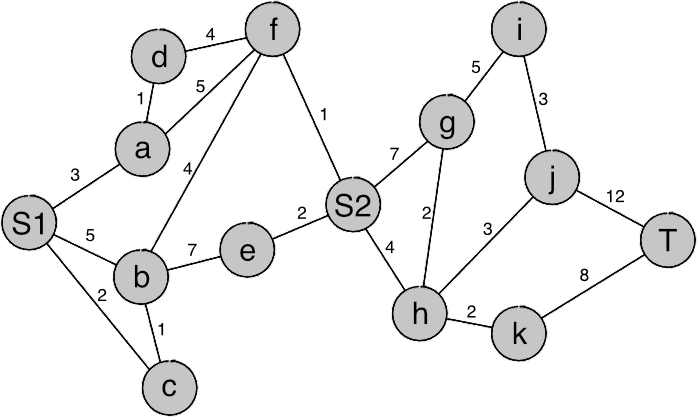
\includegraphics[scale=0.9]{chapters/informed_search/Anfangsproblem.png}
	\caption{Beispiel Graph}
\end{figure}

Wir sehen unsere Startknoten $S1$ und $S2$, sowie den Zielknoten $T$.  Au\ss erdem sind alle Kanten zwischen den Knoten mit einer L\"ange versehen. Im folgenden werden wir mit Hilfe der Breitensuche erst den Weg von $S1$ zu $T$ und dann den Weg von $S2$ zu $T$ suchen. In der folgenden Grafik sind die Zwischenknoten mit Kleinbuchstaben beschriftet, des weiteren sind Start und Ziel in gelb eingef\"arbt. In jedem Schritt werden die aktuell zu untersuchenden Knoten gr\"un und die bereits besuchten Knoten blau markiert.

\begin{figure}[h!]
	\centering
	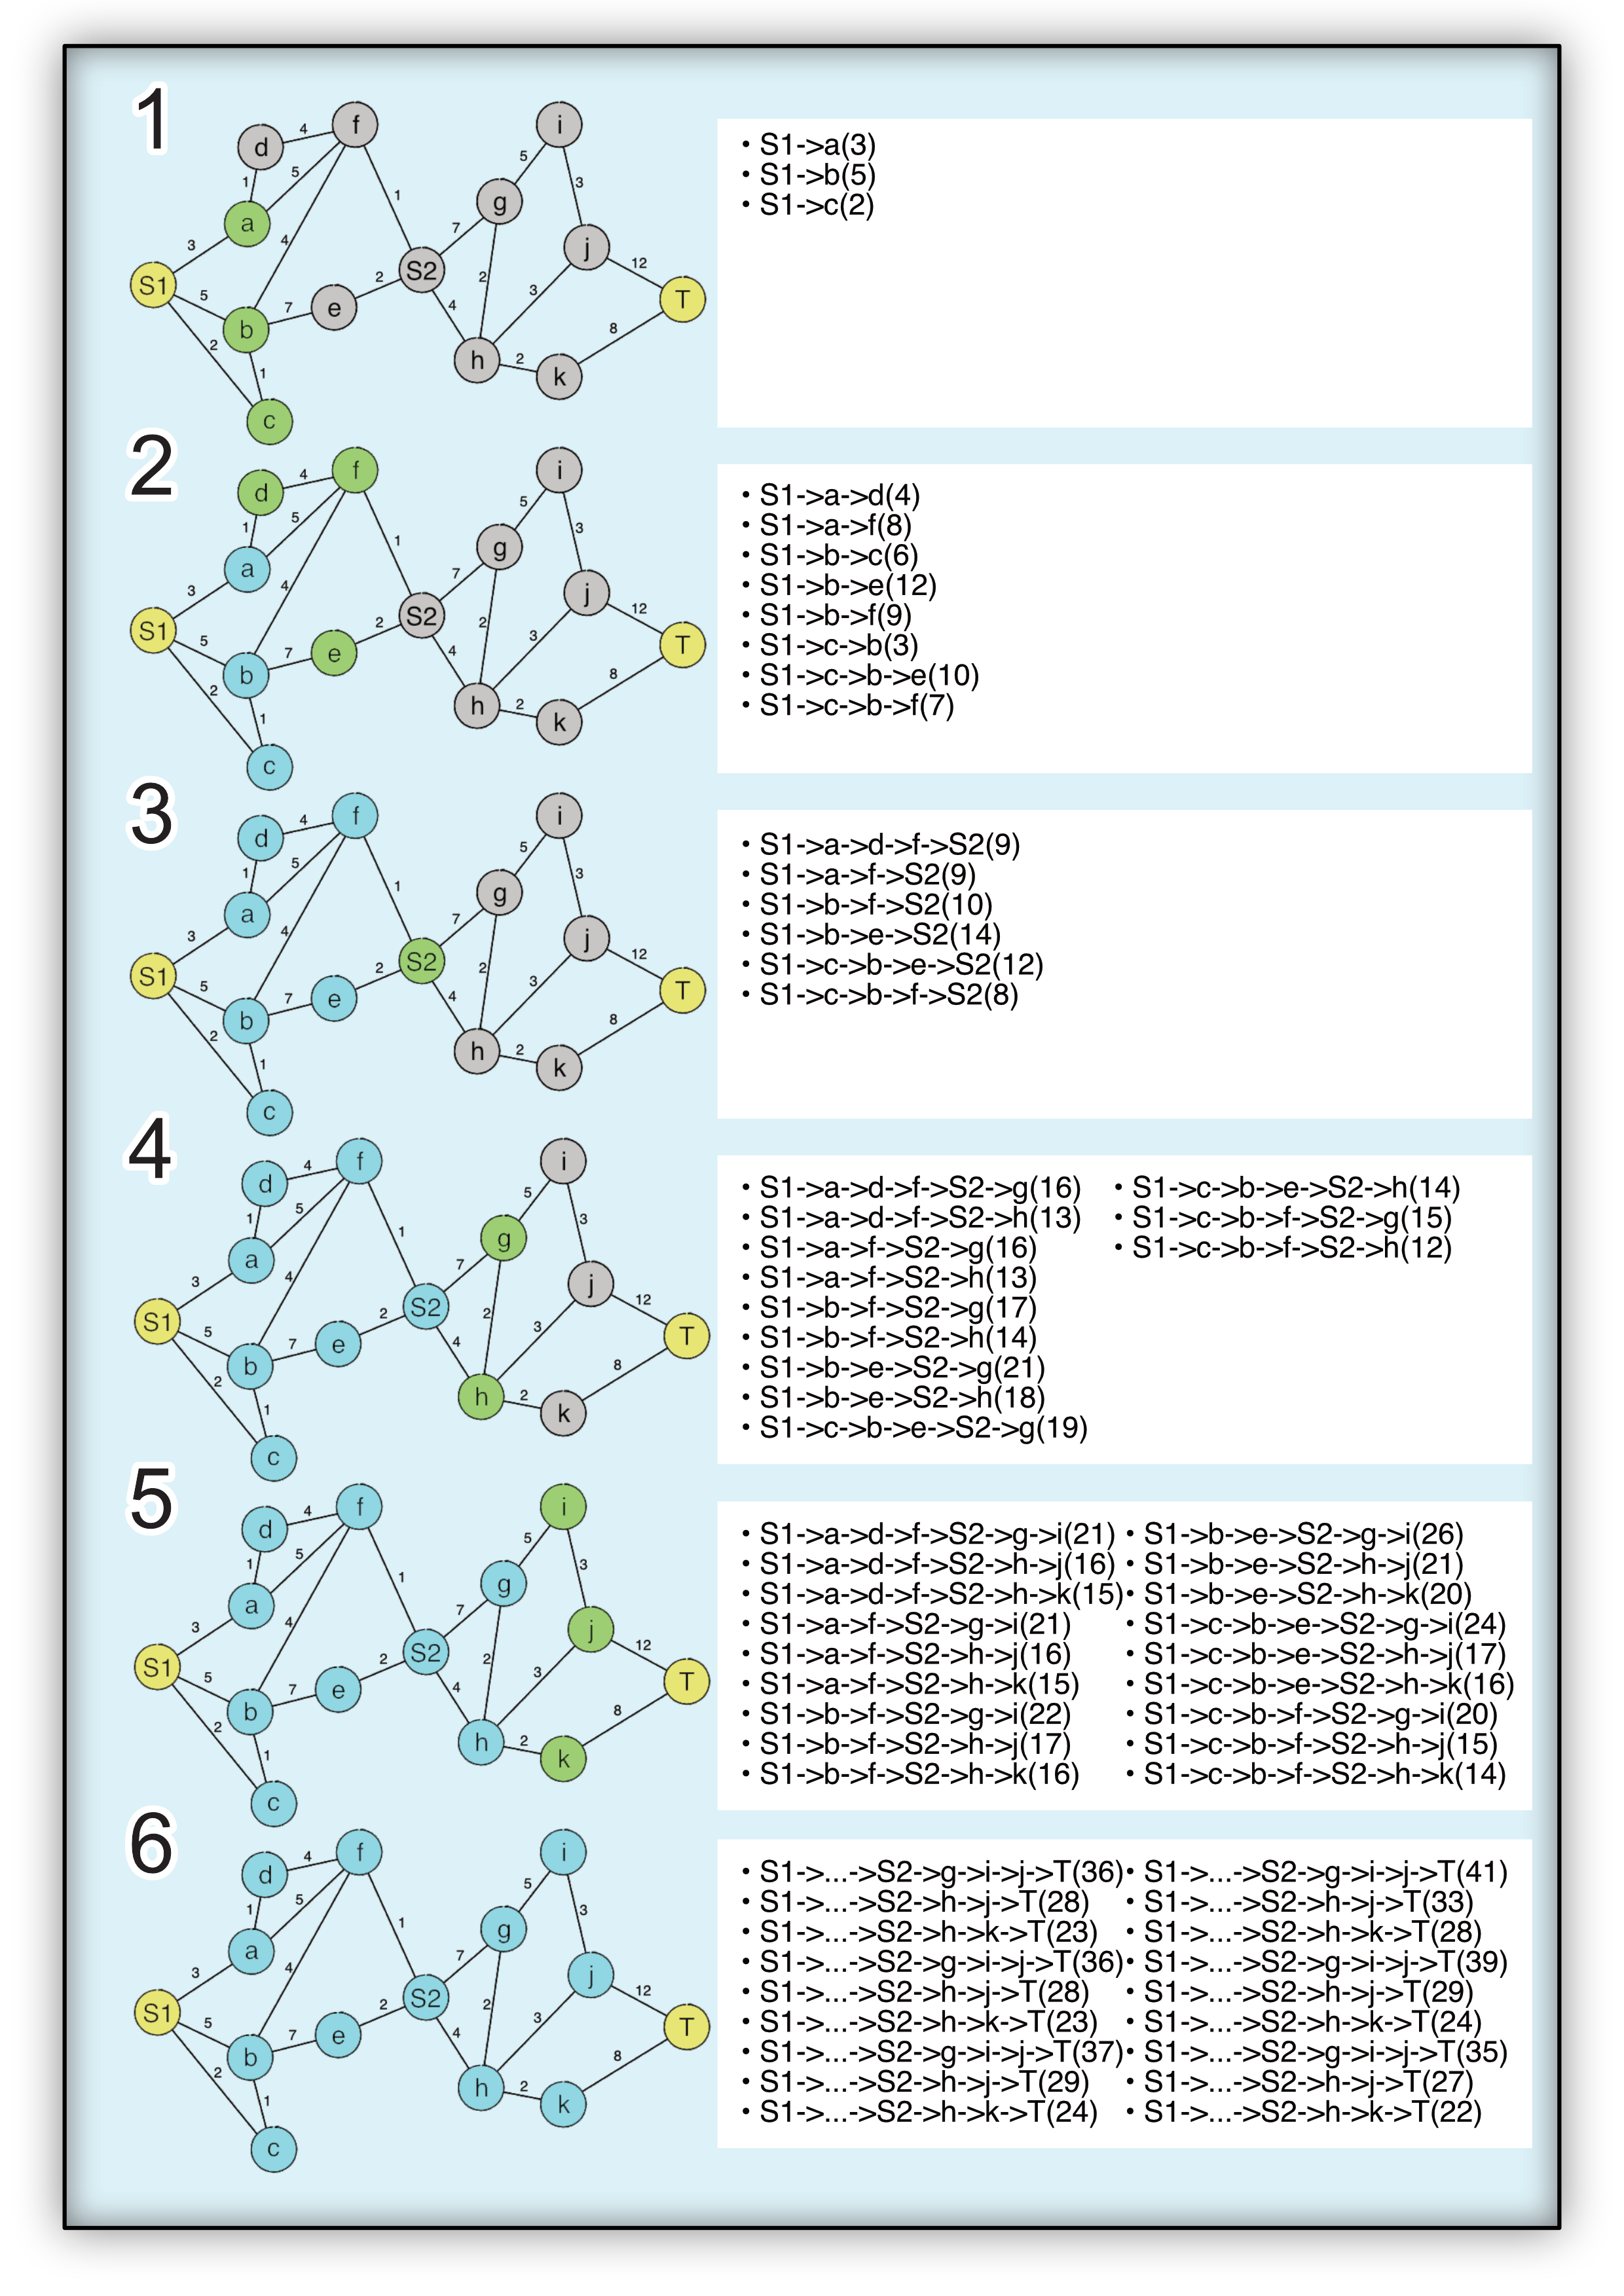
\includegraphics[scale=0.76]{chapters/informed_search/BeispielGraphen1.png}
	\caption{Beispiel Graph mit Breitensuche. Zu jedem Graphen sind die besuchten Wege angegeben. Die durch "..."\ zusammengefassten Wegst\"ucke der Wege des letzten Graphen entsprechen denen der Wegen von $S1$ nach $S2$ des vorletzten Graphens.}
\end{figure}

\begin{enumerate}
	\item Wir besuchen zuerst Knoten $a$, $b$ und $c$ und stellen offensichtlich fest, dass wir $T$ noch nicht erreicht haben. 
	\item Wir besuchen nun $d$, $e$ und $f$. Wir haben $T$ immer noch nicht erreicht.
	\item In diesem Schritt gibt es nur $S2$ zu besuchen. 
	\item Ab hier Suchen wir effektiv den k\"urzesten Weg von $S2$ zu $T$, weshalb dieses Beispiel sp\"ater nicht mehr extra erl\"autert wird. Hier besuchen wir die Knoten $g$ und $h$.
	\item Dann besuchen wir noch $i$, $j$ und $k$.
	\item Jetzt bilden wir noch die letzen Wege und diese enden beim Knoten $T$. Also sind wir fertig. 
\end{enumerate}
Der k\"urzeste Weg von $S1$ zu $T$ ist also:
\begin{itemize}
	\item  $S1\rightarrow c\rightarrow b\rightarrow f\rightarrow S2\rightarrow h\rightarrow k\rightarrow T$
\end{itemize}
Und daraus folgt der k\"urzeste Weg von S2 zu T ist: 
\begin{itemize}
	\item $S2\rightarrow h\rightarrow k\rightarrow T$
\end{itemize}
Fazit:

Wie man sieht ist das Problem gut l\"osbar mit uninformierte Suche, aber es f\"allt sofort auf das wir alle Knoten besuchen mussten und alle Wege bilden mussten.
Dies hat nicht nur hohe Speicherkosten zur Folge, sondern auch eine hohe Laufzeit. 
Bereits bei diesen simplen Beispiel sieht man die enorme Menge von Wegen die man speichern muss. 
Als Mensch w\"urde man bei dieser Suche weniger Wege betrachten:
\begin{itemize}
	\item W\"are es nicht einfacher Wege auszulassen die offensichtlich zu lang sind?
	\item Oder w\"are es nicht besser Wege wie $S1\rightarrow b$ durch den k\"urzeren $S1\rightarrow c\rightarrow b$ zu ersetzen?
\end{itemize}
Unterbewusst benutzt man eine Menge Vereinfachungen die der Computer vielleicht auch anwenden sollte. 
Im folgenden Kapitel werden wir versuchen diese Suche intuitiv zu optimieren. /newpage

\section{Verbesserungen}
\subsection{Intuitiver Algorithmus}
Statt alle Knoten zu besuchen wie bisher, werden wir im folgenden unser Wissen \"uber den Graphen nutzen um schneller zum Ergebnis zu kommen. Folgende Regeln werden angewandt:
\begin{enumerate}
	\item Wir besuchen immer den Knoten mit der niedrigsten Kantenl\"ange zuerst.
	\item Wenn wir einen neuen Weg zu einem Knoten finden und dieser k\"urzer ist als der vorherige, brauchen wir nur noch diesen neuen Weg zu betrachten. Ansonsten kann der neue Weg ignoriert werden.
	\item Wenn wir zwei Wege zur Auswahl haben, die gleichlang sind, w\"ahlen wir zuf\"allig.
	\item Wenn ein Weg keine nicht besuchten Kinder mehr hat gehen wir zur\"uck zum letzten Knoten der noch offene Kinder hatte.
	\item Aufgrund der oben genannten Regeln muss der erste Weg zum Ziel der k\"urzeste sein. (Um das Beispiel nicht unn\"otig lang zu machen, wird dies an dieser Stelle nicht bewiesen)
\end{enumerate}

\subsection{Anwendung}
Wir beginnen mit dem Graphen aus Kapitel 1. Die Knoten werden genau wie bereits bekannt eingef\"arbt werden. 

\begin{figure}[h!]
	\centering
	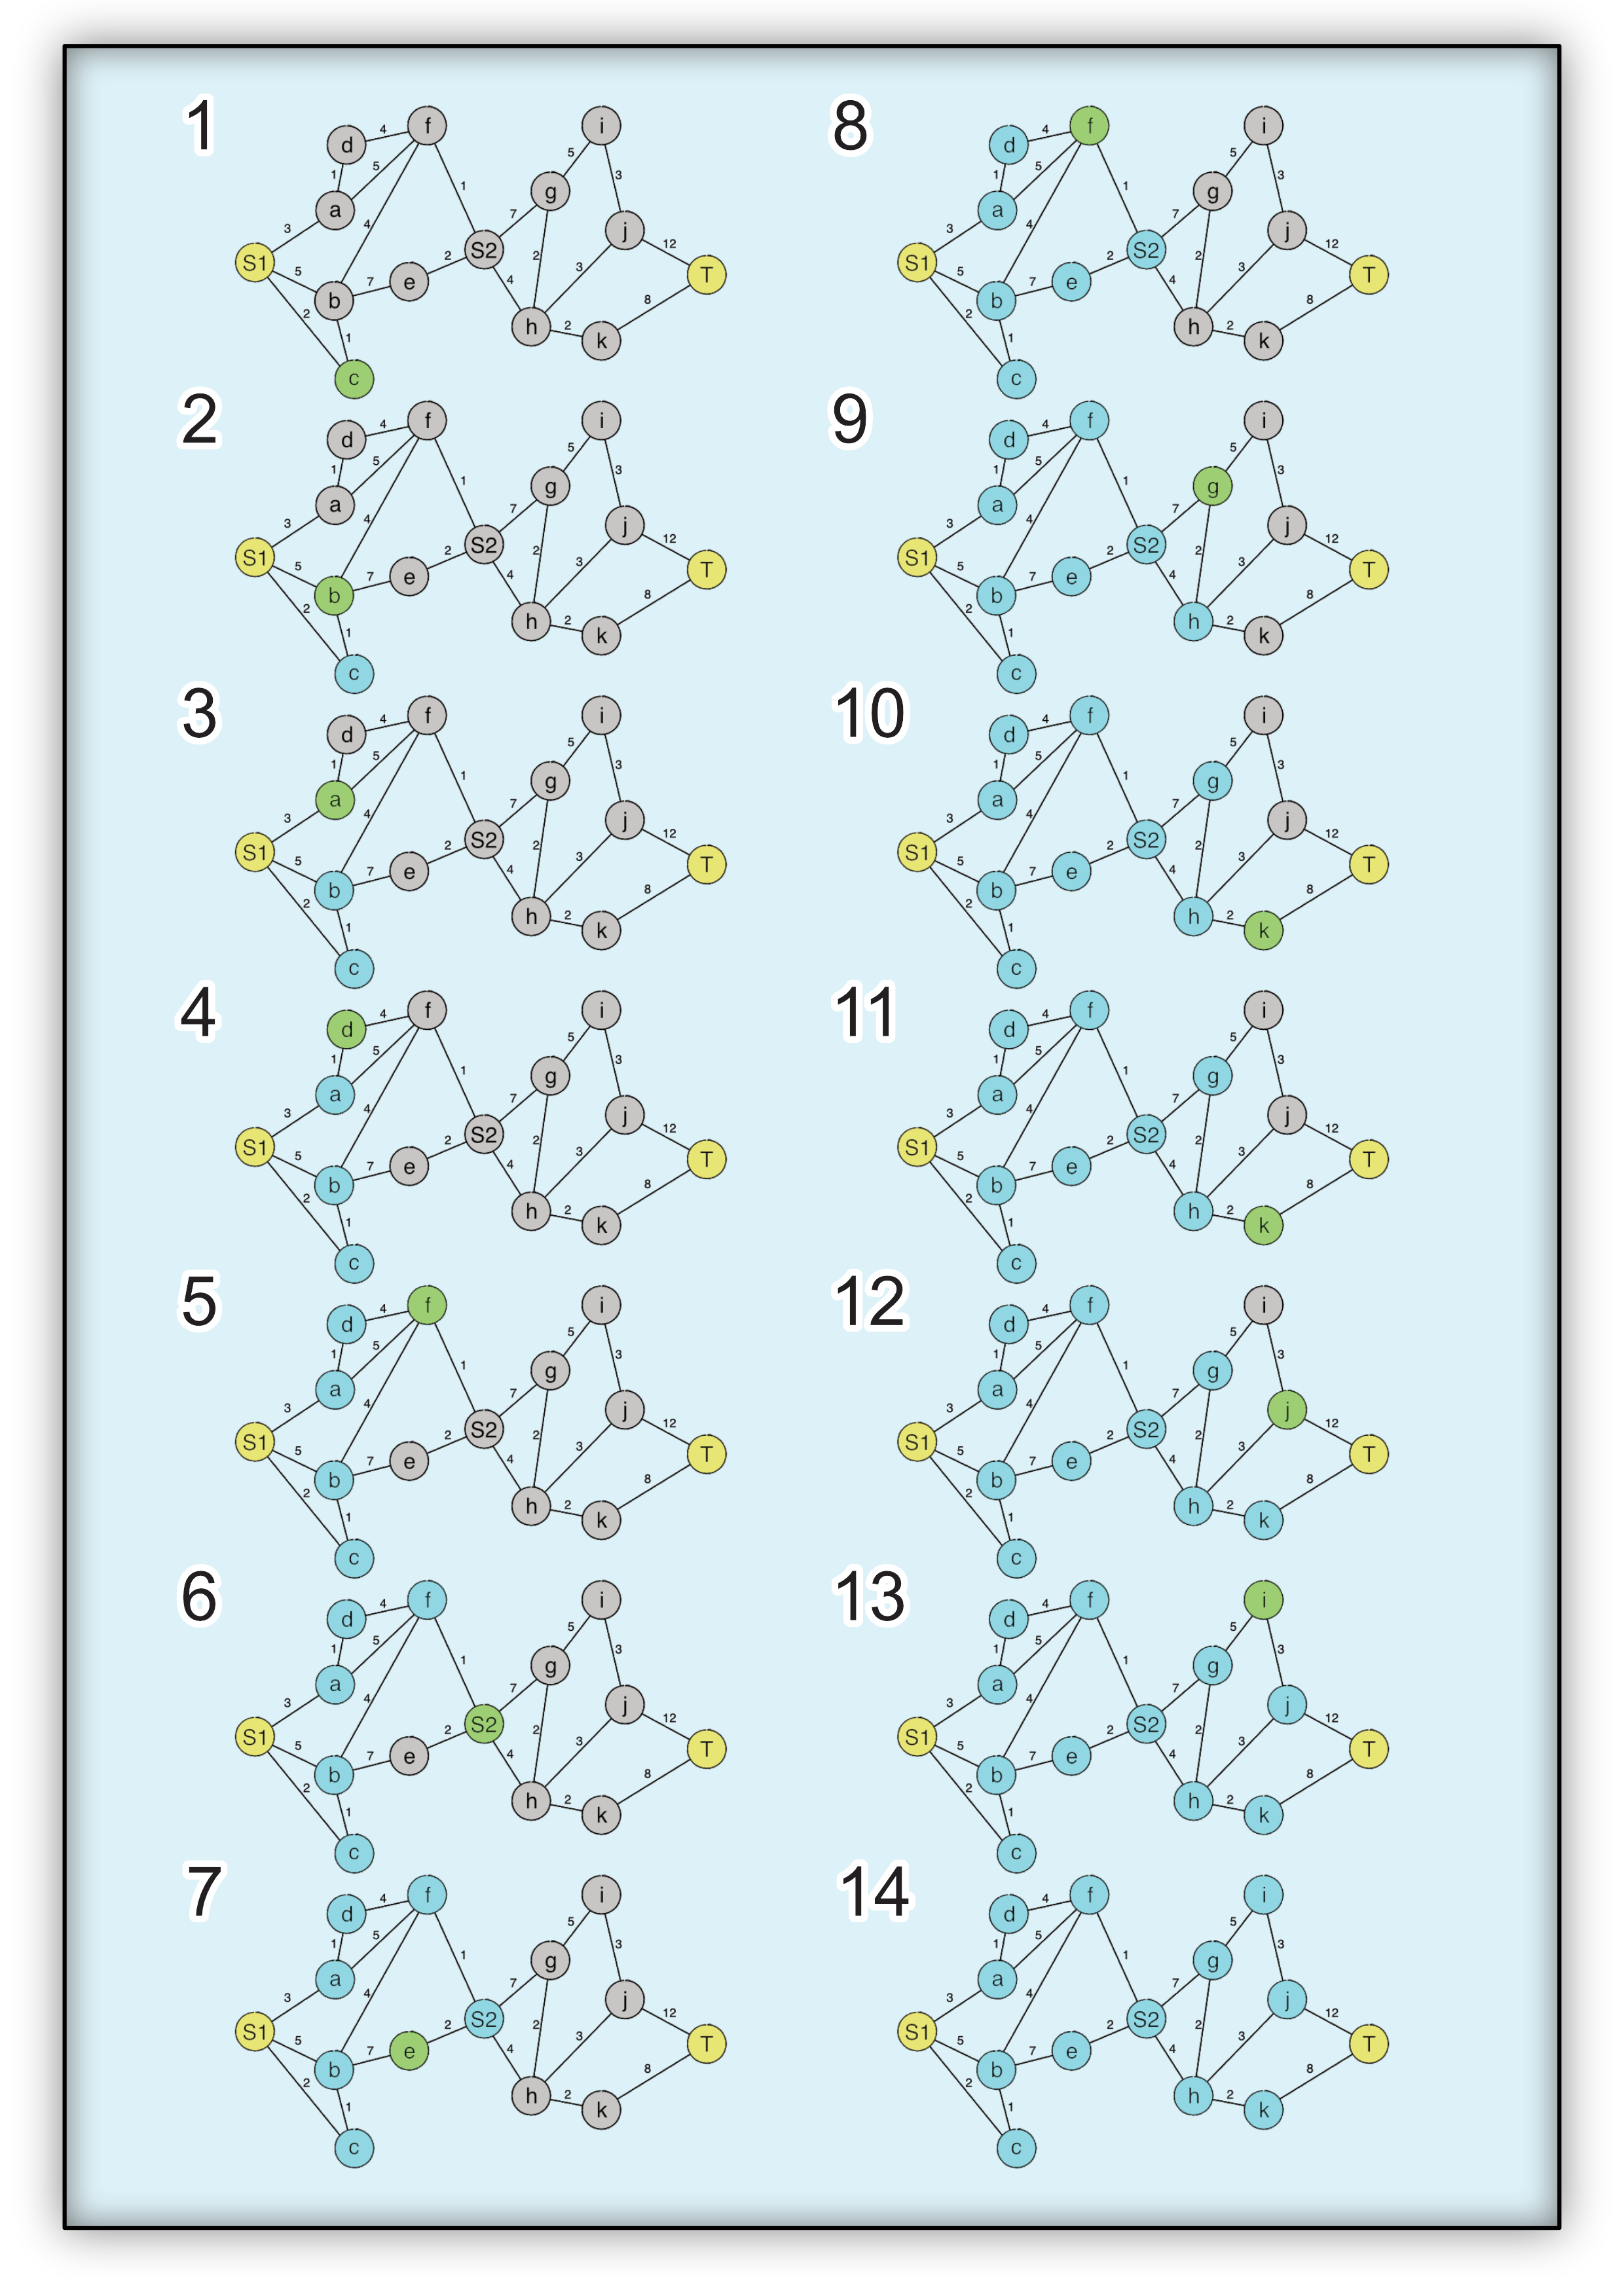
\includegraphics[scale=0.76]{chapters/informed_search/BeispielGraphen2.png}
	\caption{Beispiel Graph mit intuitiven Algorithmus.}
\end{figure}

\begin{enumerate}	\item Wir beginnen mit Knoten $c$ da mit einer L\"ange von $2$ seine Kante am k\"urzesten ist $(Regel 1)$. 
Wir haben also den Weg:
	\begin{itemize}
		\item $S1\rightarrow c(2)$
	\end {itemize}
	\item Nun besuchen wir $b$ und erhalten den Weg:
	\begin{itemize}
		\item $S1\rightarrow c\rightarrow b(3)$
	\end{itemize}
	\item Jetzt m\"ussen wir erst $a$ betrachten, da die Kante mit einer L\"ange von $3$ k\"urzer ist als $b\rightarrow f$ mit $4$. Wir haben also die Wege:
	\begin{itemize}
		\item $S1\rightarrow c\rightarrow b(3)$
		\item $S1\rightarrow a(3)$
	\end{itemize}
	\item Als n\"achstes besuchen wir $d$, da $a\rightarrow d$ am k\"urzesten ist. Es werden die Wege:
	\begin{itemize}
		\item $S1\rightarrow c\rightarrow b(3)$
		\item $S1\rightarrow a\rightarrow d(4)$
	\end{itemize}
	gespeichert.	\item Wir mussten uns zwischen $d\rightarrow f$ und $b\rightarrow f$ entscheiden und haben zuf\"allig $d\rightarrow f$ gew\"ahlt $(Regel 3)$. Damit ergeben sich die Wege:
	\begin{itemize}
		\item $S1\rightarrow c\rightarrow b(3)$
		\item $S1\rightarrow a\rightarrow d\rightarrow f(8)$
	\end{itemize}
	\item Im n\"achsten Schritt w\"ahlen wir $f\rightarrow S2$. Die Wege sind:
	\begin{itemize}
		\item $S1\rightarrow c\rightarrow b(3)$
		\item $S1\rightarrow a\rightarrow d\rightarrow f\rightarrow S2(9)$
	\end{itemize}
	\item Jetzt besuchen wir $e$. Wir haben also die Wege:
	\begin{itemize}
		\item $S1\rightarrow c\rightarrow b(3)$
		\item $S1\rightarrow a\rightarrow d\rightarrow f\rightarrow S2\rightarrow e(11)$
	\end{itemize}
	Stellen aber fest, dass $e$ f\"ur den n\"achsten Schritt keine unbesuchten Kinder hat. Also gehen wir zur\"uck zu $S2$ da dieser noch Kinder hatte $(Regel 4)$. Die Wege werden wieder zu:
	\begin{itemize}
		\item $S1\rightarrow c\rightarrow b(3)$
		\item $S1\rightarrow a\rightarrow d\rightarrow f\rightarrow S2(9)$
	\end{itemize}
	Wir besuchen noch einmal $f$, dieses Mal als $b\rightarrow f$ (zuf\"allig gew\"ahlt aus $b\rightarrow f$ und $S2\rightarrow h$). Damit haben wir einen neuen Weg zu $f$, der k\"urzer ist als $S1\rightarrow a\rightarrow d\rightarrow f$. Wir ersetzen ihn $(Regel 2)$. Damit ergibt sich der Weg:
	\begin{itemize}
		\item $S1\rightarrow c\rightarrow b\rightarrow f\rightarrow S2(8)$
	\end{itemize}	\item Wir w\"ahlen $h$ und erhalten den Weg:
	\begin{itemize}
		\item $S1\rightarrow c\rightarrow b\rightarrow f\rightarrow S2\rightarrow h(12)$
	\end{itemize}
	\item Aus $h\rightarrow g$ und $h\rightarrow k$ w\"ahlen wir $g$. Der Weg ist:
	\begin{itemize}
		\item $S1\rightarrow c\rightarrow b\rightarrow f\rightarrow S2\rightarrow h\rightarrow g(14)$
	\end{itemize}
	\item Wir besuchen $k$. Damit ergeben sich die Wege:
	\begin{itemize}
		\item $S1\rightarrow c\rightarrow b\rightarrow f\rightarrow S2\rightarrow h\rightarrow g(14)$
		\item $S1\rightarrow c\rightarrow b\rightarrow f\rightarrow S2\rightarrow h\rightarrow k(14)$
	\end{itemize}
	\item Wir w\"ahlen $j$ und erhalten die Wege: 
	\begin{itemize}
		\item $S1\rightarrow c\rightarrow b\rightarrow f\rightarrow S2\rightarrow h\rightarrow g(14)$
		\item $S1\rightarrow c\rightarrow b\rightarrow f\rightarrow S2\rightarrow h\rightarrow k(14)$
		\item $S1\rightarrow c\rightarrow b\rightarrow f\rightarrow S2\rightarrow h\rightarrow j(15)$
	\end{itemize}	\item Jetzt besuchen wir erst $j\rightarrow i$. 
	\item Dann besuchen wir sofort $g\rightarrow i$, aber wir haben \"uber $j$ bereits einen k\"urzeren Weg zu $i$ und k\"onnen den neuen ignorieren. Es folgen die Wege:
	\begin{itemize}
		\item $S1\rightarrow c\rightarrow b\rightarrow f\rightarrow S2\rightarrow h\rightarrow k(14)$
		\item $S1\rightarrow c\rightarrow b\rightarrow f\rightarrow S2\rightarrow h\rightarrow j\rightarrow i(18)$
	\end{itemize}
	Und wir sehen, dass $i$ keine Kinder mehr hat:
	\begin{itemize}
		\item $S1\rightarrow c\rightarrow b\rightarrow f\rightarrow S2\rightarrow h\rightarrow k(14)$
		\item $S1\rightarrow c\rightarrow b\rightarrow f\rightarrow S2\rightarrow h\rightarrow j(15)$
	\end{itemize}
	\item Als letztes nehmen wir noch $k \rightarrow  T$. Wir bekommen also den Weg:
	\begin{itemize}
		\item $S1 \rightarrow  c \rightarrow  b \rightarrow  f \rightarrow  S2 \rightarrow  h \rightarrow  k \rightarrow  T (22)$ 
	\end{itemize}
	und aus $Regel 5$ folgt, dass dies der k\"urzeste Weg sein muss. 
\end{enumerate}
Fazit:

Zuallererst unser Ergebnis ist identisch mit dem aus Kapitel 1, wir haben also ebenfalls den besten Weg gefunden.  Es es leicht sichtbar, dass unser intuitiver Algorithmus nicht perfekt ist. Wir mussten trotzdem alle Knoten besuchen, genau wie die Breitensuche. Aber man sieht ebenfalls sofort, dass wir deutlich weniger Wege betrachten und speichern mussten als zuvor. Und besonders hervorzuheben ist, dass wir die Suche beenden konnten als wir den ersten Weg gefunden hatten. Das wirkt sich nat\"urlich positiv auf Laufzeit und Speicherverbrauch aus. In den folgenden Kapiteln wollen wir die hier intuitiv erarbeiteten Konzepte formal definieren, die echten Algorithmen der informierten Suche vorstellen und deren Eigenschaften \"uberpr\"ufen. 
 
\section{Einleitung}
Statt blind alle M\"oglichkeiten zu probieren um die Beste zu erhalten, zieht man, wie ein Mensch es intuitiv machen w\"urde, weitere Informationen \"uber das Problem zurate (Heuristiken) und ignoriert L\"osungen die offensichtlich schlechter sind als bereits gefundene (Branch and Bound). Damit ergibt sich eine deutlich bessere Laufzeit, wie sie in Echtzeitanwendungen (z.B. in Spielen) n\"otig ist. Nat\"urlich stellt sich auch die Frage, ob diese einfacher erhaltene L\"osung immer noch die optimale L\"osung ist (Optimalit\"at). Im folgenden werden die Verschiedenen Arten (Best-First Search und A*) informierter Suche von und deren Vor- und Nachteile erkl\"art. 

\section{Definitionen}
\subsection{Branch and Bound}
Branch and Bound (h\"aufig abgek\"urzt mit B\&B\footnote{Branch and Bound Algorithms - Principles and Examples. Jens Clausen, March 12, 1999}) ist eine Optimierungsstrategie f\"ur Algorithmen, hier im speziellen Suchverfahren. Um nicht alle Knoten eines Baumes durchsuchen zu m\"ussen, kann man, wie bereits intuitiv oben gesehen, die Aufgabe in Teile aufteilen ("Branch"\ engl. "to branch" verzweigen\footnote{www.dict.cc}) und diese Teile nach Relevanz f\"ur die L\"osung einteilen ("Bound\ engl. "to bound" beschr\"anken\footnote{www.dict.cc}). 
Damit man dies bei Suchalgorithmen bewerkstelligen kann benutzt man eine Absch\"atzung, intuitiv war dies "k\"urzeste Luftlinie zum Ziel"\, auch Heuristik genannt.\footnote{Anwendungen von Branch and Bound, Frederik Wollny und Philipp Schmid, Hochschule Aalen, 2016}

\subsection{Extended List}
Bei der Anwendung von Branch and Bound kann es dazu kommen, dass Wege p'=(\dots, A) zu einen Knoten A weiter verfolgt werden, f\"ur die es einen Weg p=(\dots, A) gibt, so dass gilt:
\begin{center} 
$Wf(p) < Wf(p')$
\end{center}
Dies f\"uhrt dazu, dass der Suchbaum unn\"otig gro\ss wird. Um zu erreichen, dass nicht die l\"angeren Wege weiter verfolgt werden, wird die Extended List eingef\"uhrt. In der Extended List wird f\"ur jeden Knoten zum Zeitpunkt an dem dieser besucht wird, die Knoten Identifikation und die Wegl\"ange zu diesem gespeichert. F\"uhrt nun im Verlauf der Suche ein Weg zu einem Knoten, der bereits in der Extended List gespeichert ist, so wird die gespeicherte mit der Aktuellen Wegl\"ange zum Knoten verglichen. Ist die Aktuelle Wegl\"ange gr\"o\ss er, muss der Weg nicht weiter verfolgt werden, es gibt bereits einen k\"urzeren Weg zu dem Knoten. Ist sie geringer, wird der neue Wert eingetragen und der \"altere Weg \"uber diesen Knoten muss nicht weiter betrachtet werden.\footnote{https://ocw.mit.edu/courses/electrical-engineering-and-computer-science/6-034-artificial-intelligence-fall-2010/lecture-videos/lecture-5-search-optimal-branch-and-bound-a/} Mit Branch and Bound + Extended List ergibt sich in unserem Beispiel Graphen:

\begin{figure}[h!]
	\centering
	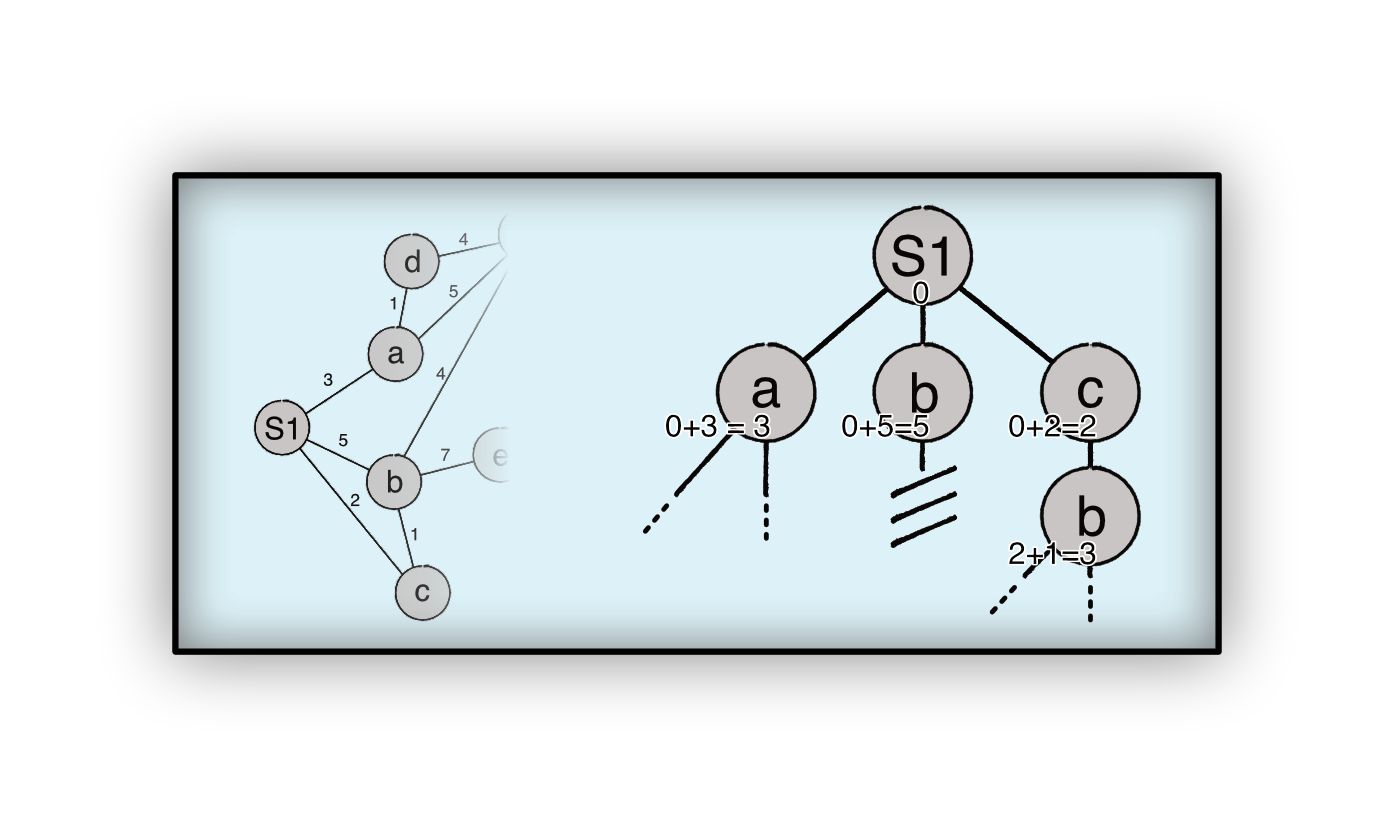
\includegraphics[scale=0.4]{chapters/informed_search/ExtendedListBeispiel.png}
	\caption{Links ist der linke Teil des Beispiel Graphen abgebildet, rechts ein Teil des Suchbaums von Branch and Bound + Extended List. Wie abgebildet wird der Weg (S1, b, \dots) nicht weiter verfolgt, da, $Wf((S1, c, b)) < Wf(S1,b)$.}
\end{figure}

\section{Best-First Search}
Best-First Search ist eine Klasse von informierten Such-Algorithmen, welche nachdem Prinzip arbeiten, dass sie stets denjenigen Knoten zuerst untersuchen, welcher f\"ur den Erfolg der Suche am "vielversprechendsten"\ erscheint. Die Wahl dieses "vielversprechenden"\ Knotens geschieht anhand einer gewissen Heuristik. Der wohl bekannteste Algorithmus aus diesem Bereich ist A*, welcher auch als eine Erweiterung von Branch and Bound gesehen werden kann. An ihm wollen wir im Folgenden das Prinzip von Best-First Search verdeutlichen. 

\section{Heuristik}
Die Heuristik ist im Falle der Informierten Suche die Representation der menschlichen L\"osungsfindung im Such-Algorithmus. Sie weist jedem Knoten einen gesch\"atzten Wert zu, der dar\"uber Auskunft gibt, ob es sich lohnen k\"onnte, einen Weg \"uber diesen Knoten einzuschlagen. Bei der Findung des k\"urzesten Weges gilt, desto h\"oher der durch die Heuristik bestimmte Wert f\"ur einen Knoten ist, desto unwahrscheinlicher ist es, dass der K\"urzeste Weg \"uber diesen Knoten verl\"auft. Aufgrund der Vielfalt von Gegebenheiten unter denen eine Suche stattfinden kann, ist es offensichtlich, dass eine Heuristik die ein Problem L\"ost nicht ohne weiteres auf andere Probleme \"ubertragen werden kann. Deswegen werden zun\"achst einige wichtige Begrifflichkeiten gekl\"art, die beim Umgang mit Heuristiken helfen k\"onnen.\footnote{http://www.duden.de/rechtschreibung/Heuristik}

\subsection{Eigenschaften von Heuristiken}
Im folgenden werden einige Eigenschaften definiert, die eine Heuristikfunktion erf\"ullen kann. Diese Eigenschaften k\"onnen dabei helfen ein Urteil, \"uber die Zul\"assigkeit einer Heuristik f\"ur eine Problemstellung, zu f\"allen.
\newtheorem*{theore}{Theorem}
\theoremstyle{definition}
\newtheorem*{defi}{Definition}

\begin{defi}
Eine heuristische Funktion $h(n)$ wird als admissible (zul\"assig) bezeichnet, wenn f\"ur alle Knoten $n$ erf\"ullt ist: 
\begin{center}
$h(m) \leq k(m, n)$
\end{center}
mit $k(m, n)$ als k\"urzeste Wegl\"ange von $m$ nach $n$ und f\"ur alle Knoten $t \in G$, die die Endbedingung erf\"ullen, gilt: 
\begin{center}
$h(t)=0.\footnote{https://ocw.mit.edu/courses/electrical-engineering-and-computer-science/6-034-artificial-intelligence-fall-2010/lecture-videos/lecture-5-search-optimal-branch-and-bound-a/}$
\end{center}
\end{defi}

Admissible Heuristiken reichen bereits aus, um auf Landkarten o.\"a. nach der k\"urzesten Route zu suchen. Damit eine Heuristik auch f\"ur Suchen verwendet werden kann die nicht auf geografischer Ebene stattfinden, werden die Eigenschaften konsistent und monoton definiert. Die Definitionen wurden aus [Kai13] \"ubernommen. 

\begin{defi}
Eine heuristische Funktion $h(n)$ ist konsistent, wenn f\"ur alle Knotenpaare $m, n \in G$ folgendes erf\"ullt ist: 
\begin{center}
$h(m) \leq k(m, n) + h(n)$
\end{center}
mit $k(m, n)$ als k\"urzeste Wegl\"ange von $m$ nach $n$ und f\"ur alle Knoten $t \in G$, die die Endbedingung erf\"ullen, gilt: 
\begin{center}
$h(t)=0$.
\end{center}
\end{defi}

\begin{defi}
Eine heuristische Funktion $h(n)$ ist monoton, wenn f\"ur alle Knotenpaare $m, n \in G$ mit $n$ als unmittelbarem Nachbar von $m$ folgendes erf\"ullt ist: 
\begin{center}
$h(m) \leq c(m, n) + h(n)$
\end{center}
mit $c(m, n)$ als Kosten der Kante von $m$ nach $n$; und f\"ur alle Knoten $t \in G$, die die Endbedingung erf\"ullen, gilt: 
\begin{center}
$h(t)=0$.
\end{center}
\end{defi}

\begin{theore}
Die Eigenschaften konsistent und monoton sind \"aquivalent.
\end{theore}

\begin{theore}
F\"ur jede konsistente Funktion $h$ gilt:
$h(n) \leq h*(n)$ f\"ur alle Knoten $n \in G$.
\end{theore}

Um den unterschied zwischen einer Heuristik die admissible ist und einer die konsistent ist zu verdeutlichen, sei ein Beispiel angef\"uhrt: 

\begin{figure}[h!]
	\centering
	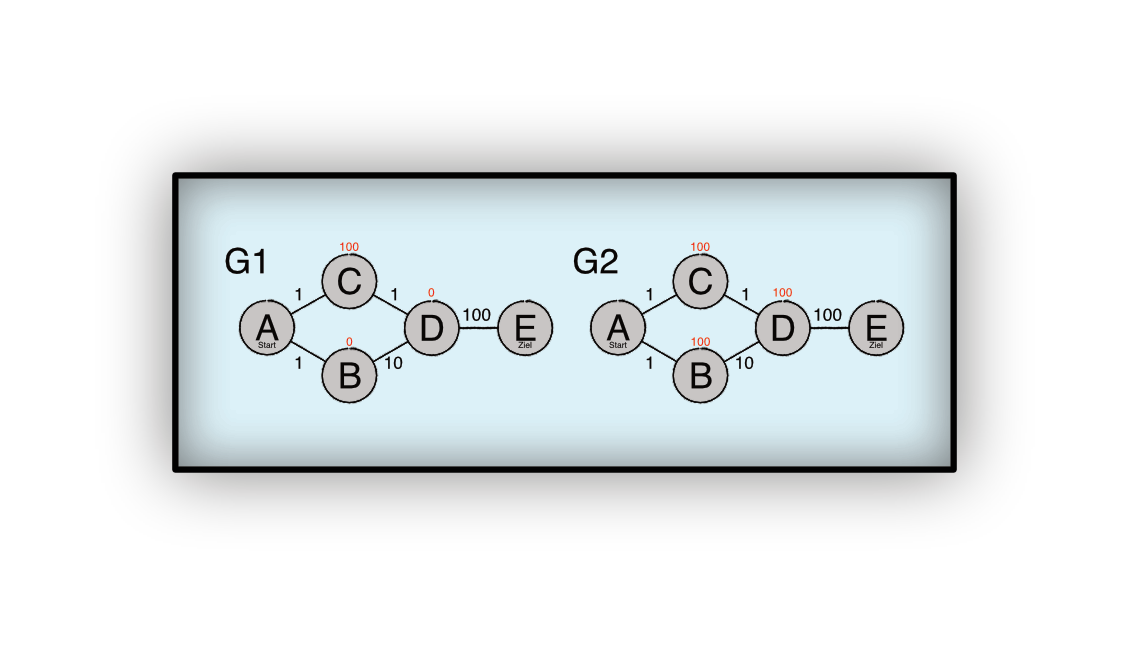
\includegraphics[scale=0.5]{chapters/informed_search/BeispielHeuristik.png}
	\caption{Die Abbildungen G1 und G2 beschreiben das selbe Problem mit zwei verschiedenen Heuristiken. Ziel ist es den k\"urzesten Weg von Knoten A nach Knoten E zu finden. G1 stellt die Verwendung einer admissible Heuristik und G2 die einer konsistenten Heuristik dar. Die roten Zahlen geben die Werte der Heuristikfunktionen an den relevanten Knoten an. Wird nun eine Suche, mit Branch and Bound + Extended List + Heuristik durchgef\"uhrt, liefert die Suche f\"ur G1 den Weg(A,B,D,E) und f\"ur G2 den Weg(A,C,D,E). Entscheidend f\"ur diese L\"osung ist, dass bei G1 zun\"achst A,B, und D betrachtet werden und somit aufgrund der Extended List der Weg (A,C,D,E) wegf\"allt. Im Gegensatz dazu beginnt die Suche bei G2 mit einem Weg \"uber C, da die gesch\"atzten Kosten von C mit 101 kleiner als die von B sind.}
\end{figure}

\subsection{Verschiedene Heuristiken}
In diesem Abschnitt werden drei Heuristiken vorgestellt, angefangen mit der Hamming-Distanz. Aufgrund dessen, dass in einigen Kapiteln Bezug auf die folgenden Heuristiken genommen wird, wurden einige Bezeichnungen in den Definitionen entsprechend angepasst.\\
Die Hamming-Distanz hh(m,n) beschreibt wie gro\ss der Unterschied zwischen den Zeichenketten m und n ist und ist wie folgt definiert: 
\begin{defi}
$\sum$ sei ein endliches Alphabet sowie $m = (m_{1}, \dots, m_{k})$ und $y = (n_{1}, \dots, n_{k})$ zwei $k$ Zeichen lange Worte aus $\sum^{k}$. Die Hamming-Distanz zwischen $m$ und $n$ ist definiert als:
\begin{center}
$h_{h}(m,n) := |{j \in \{1 , \dots , k\} | m_{j} \neq n_{j}}|$.
\end{center}
\end{defi}
Eine Heuristik w\"are z.B. $h(n)=h_{h}(n,x)$, mit $x$ als Ziel-Konstellation der Suche.\footnote{http://sb.fluomedia.org/hamming/, https://de.wikipedia.org/wiki/Hamming-Abstand}
\begin{defi}
Die Manhattan Distanz $h_{m}(m,n)$ f\"ur die Punkte $n$ und $m$ beschreibt die Distanz, die zustande kommt, wenn nur horizontale und vertikale Wege genommen werden, um $n$ von $m$ aus zu erreichen. Die Manhattan-Distanz ist wie folgt definiert:
\begin{center}
$h_{m}(m,n) = \sum_{i} |m_{i} - n_{i}|.$
\end{center}
\end{defi}
Eine Heuristik w\"are z.B $h(n)=h_{m}(n,x)$, mit $x$ als Ziel-Knoten der Suche.\footnote{http://mathworld.wolfram.com/TaxicabMetric.html}
\begin{defi}
Der Euklidischer Abstand $h_{e}(m,n)$ von $m$ und $n$ entspricht der "Luftlinie" zwischen diesen. Der Euklidische Abstand f\"ur zwei Vektoren im $k$-Dimensionalen Raum ist wie folgt definiert:
\begin{center}
$h_{e}(m,n) =\sqrt{((m_{1} - n_{1})^{2}+\dots+(m_{k} - n_{k})^{2})}.$
\end{center}
\end{defi}
Eine Heuristik w\"are z.B $h(n)= h_{e}(n,x)$, mit $x$ als Ziel-Knoten der Suche.\footnote{http://mathworld.wolfram.com/EuclideanMetric.html}

\subsection{Findung von Bewertungsfunktionen}
Die Frage Lautet:"Wie findet sich die richtige Heuristikfunktion f\"ur die gegebene Problemstellung". Um einen L\"osungsansatz f\"ur eine allgemeine Vorgehensweise zu finden, wird zun\"achst das Beispiel aus 5.1 betrachtet. Die Aufgabe im Beispiel ist es, den k\"urzesten Weg von dem Knoten S1 bzw. S2 zum Zielknoten T im Graphen zu finden. Die Problemstellung l\"asst sich in eine Konjunktion von zwei Bedingungen aufteilen:
\begin{enumerate}
	\item Die zur\"uckgelegte Strecke von S1 bzw. S2 nach T soll minimal sein.
	\item Die Strecke entspricht einem Weg (Graphentheorie).
\end{enumerate}
W\"urde die zweite Bedingung weggelassen, w\"urde immer eine Strecke entsprechend der Luftlinie von $S1$ bzw. $S2$ nach $T$ gew\"ahlt werden. Es liegt also nahe $h(n)=h_{e}(n,x)$ zu w\"ahlen, um einem Knoten nach seiner Distanz zu $T$ zu bewerten. Wird Bedingung zwei nun hinzugezogen, werden mit der gew\"ahlten Heuristik immer die erreichbaren Knoten bevorzugt, die am n\"achsten zum Ziel liegen. So ist eine Akzeptable Heuristik f\"ur die Problemstellung gefunden. Dieses Prinzip des Konstruieren von vereinfachten Modellen durch systematisches Weglassen von Bedingungen der Konjunktion der Problemstellung scheint auch allgemein eine gute Herangehensweise zu sein, um leicht heuristische Sch\"atzungen zu ermitteln.

\section{A* Algorithmus}
A* beschreibt eine Gruppe von Algorithmen, die auf alle Kniffe der Informierten Suche, die bis jetzt vorgestellt wurden, zur\"uckgreifen:\footnote{https://ocw.mit.edu/courses/electrical-engineering-and-computer-science/6-034-artificial-intelligence-fall-2010/lecture-videos/lecture-5-search-optimal-branch-and-bound-a/}
\begin{itemize}
	\item Branch and Bound
	\item Extended List
	\item Heuristik
\end{itemize}
F\"ur ein gegebenes Problem gibt es innerhalb dieser Gruppe bessere und schlechtere Algorithmen. Um zwei A* Algorithmen zu vergleichen hilft das folgende Theorem: 

\begin{theore}
A*1 und A*2 seien zwei Versionen von A* mit $h1(n) ? h*(n)$ und $h2(n) ? h*(n)$ f\"ur alle Knoten $n \in G$ und mit $h1(n) ? h2(n)$ f\"ur alle Knoten $n \in G \ {t | t erf\"ullt die Endbedingung }$. (A*2 sei "besser informiert" als A*1.) Falls es eine L\"osung gibt, so wird bis zur Terminierung jeder von A*2 expandierte Knoten auch von A*1 expandiert, (A*2 "dominiert" A*1.)\footnote{[Kai13]} 
\end{theore}

In den folgenden Abschnitten wird auf weitere Eigenschaften des A* eingegangen und anschlie\ss end wird der A* durch Beispiele veranschaulicht. 

\subsection{Zul\"assigkeit}
Welche Bedingungen muss eine Heuristik erf\"ullen, damit unser Such-Verfahren ordnungsgem\"a\ss funktioniert? Dazu sollten wir zuerst definieren, wie wir uns ein korrekte Funktionsweise vorstellen.
\begin{itemize}
	\item Zul\"assigkeit Ein Such-Verfahren hei\ss t zul\"assig, falls es stets mit einer optimalen L\"osung terminiert, falls diese existiert.
\end{itemize}
Da bei unserem heuristischen Such-Verfahren A* die Wahl der Heuristik bisher nicht klar eingeschr\"ankt ist, liegt es nahe, dass in dieser Wahl ein entscheidender Punkt f\"ur die Zul\"assigkeit unseres Algorithmus liegt. Man kann sich leicht Heuristiken \"uberlegen, welche die Funktionsweise von A* st\"oren und daf\"ur sorgen, dass der Algorithmus keine optimale L\"osung findet oder wom\"oglich gar nicht erst terminiert. Wir sollten uns also genauer mit der Beschaffenheit von Heuristikfunktionen auseinandersetzen. Eine erste wichtige Eigenschaft einer Heuristik h zur Sch\"atzung von h* ist, ob diese optimistisch sch\"atzt.
\begin{itemize}
	\item optimistische Sch\"atzung Eine Sch\"atzung h von h* ist genau dann eine optimistische Sch\"atzung, falls sie die Kosten eines optimalen Pfades nie \"ubersch\"atzt.
\end{itemize}
Das heisst:
\begin{itemize}
	\item $h(n) \leq h*(n)$ f\"ur alle Knoten $n \in GP$
\end{itemize}

Diese Eigenschaft liefert uns nun die ausschlaggebende Bedingung f\"ur die Zul\"assigkeit von A*. Zul\"assigkeit von A*. Falls die verwendete Heuristik h eine optimistische Sch\"atzung von h* ist, dann ist A* zul\"assig. 
Der Beweis dieses Satzes und einige genauere Er\"orterungen k\"onnen in [Kai13] nachgelesen werden. 

\subsection{Komplexit\"at}
Es l\"asst sich leicht erkennen, dass A* in der Regel eine weit bessere Komplexit\"at hat, als blinde Such-Verfahren. Die Anzahl der expandierten Knoten ist bei A* oft sogar um ein Vielfaches geringer. Sei nun die L\"ange einer optimalen L\"osung mit d bezeichnet. Des Weiteren kann man von Einheitskosten ausgehen und die Existenz genau einer optimalen L\"osung voraussetzen. Je nachdem wie optimistisch nun der Fehler von h bez\"uglich h* angenommen wird, kommt man auf eine quadratische oder sogar lineare Komplexit\"at bez\"uglich d. Im eher realistischen Fall l\"asst sich jedoch nur auf eine exponentielle Komplexit\"at schliessen. 

\subsection{Optimalit\"at}
Nun interessieren wir uns f\"ur die Optimalit\"at von A* im Hinblick auf die Anzahl der expandierten Knoten. Der Begriff Optimalit\"at beruht hier auf dem der Dominanz. Das bedeutet, ein Verfahren ist optimal gegen\"uber einer Klasse von Verfahren, wenn es alle Elemente aus dieser Klasse dominiert. F\"ur den ganz allgemeinen Fall l\"asst sich leicht erkennen, dass A* nicht das optimale Verfahren \"uberhaupt ist. Es gibt in bestimmten F\"allen offensichtlich Verfahren, welche nicht alle von A* untersuchten Knoten ebenfalls untersuchen. Gerade bei speziell auf eine Klasse von Graphen abgestimmten Verfahren ist dies der Fall. Jedoch ist unter bestimmten Einschr\"ankungen eine konkretere Aussage bez\"uglich der Optimalit\"at von A* m\"oglich. Daf\"ur schr\"ankt man die Bedingungen auf eine Dom\"ane ein, welche eine konsistente Heuristik h besitzt, und setzt voraus, dass es mindestens einen optimalen L\"osungspfad gibt, bei welchem h < h* f\"ur alle Knoten au\ss er dem Zielknoten gilt. Dann gilt, dass A* dominant f\"ur alle Problem-Instanzen ist, und zwar f\"ur alle m\"oglichen Entscheidungsregeln bei Nicht-Eindeutigkeit des Knotens mit minimalem f-Wert. Da dem Algorithmus A* bei konsistentem h zus\"atzlich eine sehr gute Verwaltung des Suchbaumes m\"oglich ist, l\"asst sich sagen, dass A* unter diesen Voraussetzungen sehr effektiv ist. 

\subsection{Beispiel des 8-Puzzles}
Beim 8-Puzzle handelt es sich um ein Spiel, bestehend aus einem Spielbrett der Gr\"o\ss e 3-mal-3 und acht Kacheln, nummeriert von 1 bis 8, welche auf dem Spielbrett verteilt sind. Ein Feld des Spielbrettes bleibt also frei. Grenzt eine Kachel an dieses freie Feld, so kann sie an dessen Stelle verschoben werden. Das Ziel des Spieles ist, von einer ungeordneten Stellung der Kacheln durch eine Folge von Verschiebungen zu einer Zielstellung zu gelangen. Die folgende Abbildung zeigt ein konkretes Problem mittels Start- und Zielkonfiguration.
\begin{center}\includegraphics[scale=0.7]{chapters/informed_search/startziel.png}\end{center}
Die Problemstellung ist, zu einer gegebenen Kachelkonstellation die k\"urzeste Abfolge von Verschiebungen zu finden, die n\"otig ist, um zur Zielkonfiguration zu gelangen.

Wird das Problem abstrakt betrachtet, ist es m\"oglich einen Graphen zu konstruieren, auf den eine informierte Suche angewendet werden kann. Die Knoten des Graphen repr\"asentieren die Konstellationen die das Kachelfelde annehmen kann und zwei Knoten sind genau dann \"uber eine Kante miteinander verbunden, wenn sich die Kachelkonstellationen der Knoten um genau 1 Verschiebung unterscheidet. Als Kantenbewertung $f:E \rightarrow \Re$ wird die Anzahl der Verschiebungen gew\"ahlt die n\"otig ist, um die Kachelkonstellation des Zielknotens zu erhalten. In dem konstruierten Graphen ist die l\"ange jeder Kante 1.

Auf den so erhaltenen Graphen l\"asst sich nun eine informierte Suche mit einem A* Algorithmus durchf\"uhren. Um die Heuristik des A* leichter zu bestimmen, wird die Problemstellung in eine
Konjunktion aus den folgenden Bedingungen zerlegt:
\begin{enumerate}
	\item Die Anzahl der Verschiebungen soll minimal sein.
	\item Es d\"urfen nur Kacheln auf benachbarte Felder verschoben werden.
	\item Das benachbarte Feld muss leer sein.
\end{enumerate}
F\"ur Bedingung 1 bietet sich die Hamming-Distanz an. Diese gibt f\"ur jede Kachelkonstellation die Anzahl der falsch positionierten Felder an. Wird nun die 2 Bedingung hinzugezogen, muss ber\"ucksichtigt werden, dass keine diagonalen Z\"uge m\"oglich sind. Durch diese Versch\"arfung ist die Manhattan-Distanz eine passendere Heuristik. Die Manhattan-Distanz berechnet f\"ur eine gegebene Kachelkonstellation die Anzahl der horizontalen und vertikalen Verschiebungen, die n\"otig sind, um die Zielkonstellation zu erhalten. Wird zuletzt noch die 3 Bedingung hinzugezogen kann bei der Manhattan Distanz verblieben werden. Nichts desto trotz k\"onnen beide Heuristiken f\"ur das Problem verwendet werden und dies wird auch getan. Im folgenden bezeichnet die Heuristikfunktion\dots 
\begin{itemize}
	\item $h_{1}(n)$, die Anzahl falsch positionierter Kacheln in der durch Knoten n dargestellten Konfiguration (Hamming-Distanz)
	\item $h_{2}(n)$, die Summe der Distanzen der falsch positionierten Kacheln zu ihrer Zielposition (Manhattan-Distanz)
\end{itemize}
Der Ablauf des Algorithmus unter Verwendung von $h_{1}(n)$ bzw. $h_{2}(n)$ wird durch die Suchb\"aume $G_{S1}$ bzw. $G_{S2}$ dargestellt. $g$ bezeichnet die zur\"uckgelegte Wegstrecke, $h$ den Wert von $h_{1}(n)$ bzw. $h_{2}(n)$ f\"ur die gegebene Kachelkonstellation und $f$ die Summe von $h$ und $g$.

Wie an den folgenden beiden Suchb\"aumen zu sehen, ben\"otigt der A* Algorithmus unter Verwendung von $h_{2}(n)$ eine geringere Anzahl von Expansionen als bei der Verwendung von $h_{1}(n)$ ). Der Aufwand ist also geringer. Die Wahl des zu expandierenden Knotens ist stets eindeutig. Heuristik $h_{2}(n)$ scheint also ein besserer Sch\"atzer zu sein als $h_{1}(n)$. 
\begin{figure}[h!]
	\centering
	\includegraphics[scale=0.45]{chapters/informed_search/tree1.png}
	\caption{Suchbaum $G_{S1}$ zu $h_{1}$}
\end{figure}
\begin{figure}[h!]
	\centering
	\includegraphics[scale=0.65]{chapters/informed_search/tree2.png}
	\caption{Suchbaum $G_{S2}$ zu $h_{2}$}
\end{figure} 
\subsection{A* am Beispiel Graphen}
Abschlie\ss end soll ein A* Algorithmus f\"ur das in Abschnitt 6.1 pr\"asentierte Problem entworfen werden. Branch and Bound + Extended List wird wie beschrieben verwendet, die Heuristikfunktion 
\begin{center}
$h(n) = h_{e}(n,x) =sqrt((n^{1} - x^{1})^{2}+\dots+(n^{k} - x^{k})^{2})$, mit $x$ als Ziel-Knoten der Suche, 
\end{center}
wird f\"ur die Problemstellung \"ubernommen. Da es sich um die vereinfachte representation einer Karte handelt, wird $k=2$ gew\"ahlt. Der resultierende Graph mit den in rot durch die Heuristik bestimmten Werten: 

\begin{figure}[h!]
	\centering
	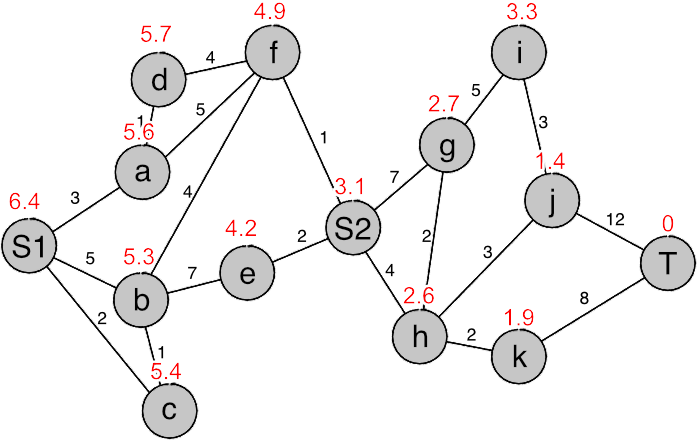
\includegraphics[scale=0.9]{chapters/informed_search/AnfangsproblemHeuristik.png}
	\caption{Beispiel Graph mit Heuristik}
\end{figure}

F\"ur die Suche des k\"urzesten Weges von S1 bzw. S2 nach T ergeben sich die beiden Suchb\"aume B1 (Abbildung6.9) und B2 (Abbildung6.10). Die in blau gekennzeichneten Zahlen geben die Reihenfolge an in der die Pfade begangen werden. Rote Zahlen geben den von der Heuristik gesch\"atzten Wert f\"ur den entsprechenden Knoten an. Die Schwarzen Zahlen geben die tats\"achliche Wegl\"ange vom Startknoten zum betrachteten Knoten an. In lila werden die gesch\"atzten Gesamtkosten eines Knotens angegeben. Als Grau markierte Pfade wurden aufgrund der Extended List ausgeschlossen.

An beiden Suchb\"aumen ist gut zu erkennen, dass viele Abzweigungen aufgrund der Extended List nahezu sofort abgeschnitten werden (gekennzeichnet durch graue Pfade). Am Baum mit Wurzel S2 l\"asst sich der nutzen einer Heuristik nachvollziehen. Die Kosten der Abzweigungen e, f in den linken Teil des Graphen nehmen durch die Heuristik schneller zu und dies sorgt daf\"ur, dass eine Suche dort obsolet (auch durch graue Pfade gekennzeichnet) wird, sobald die gesch\"atzten Kosten gr\"o\ss er als 14 sind (Der k\"urzeste Weg von S2 nach T hat die l\"ange 14). 
Die unterschiedliche Struktur der B\"aume l\"asst sich durch den Startpunkt der Suche erkl\"aren. Aufgrund dessen, dass die Knoten S1 und T auf entgegengesetzten Seiten des Graphen liegen, ergibt sich ein tiefer Baum und da der Knoten S2 den Graphen in zwei Partitionen auftrennt, bildet sich bei der Suche des k\"urzesten Weges von S2 nach T ein breiter Suchbaum. 
\begin{figure}[h!]
	\centering
	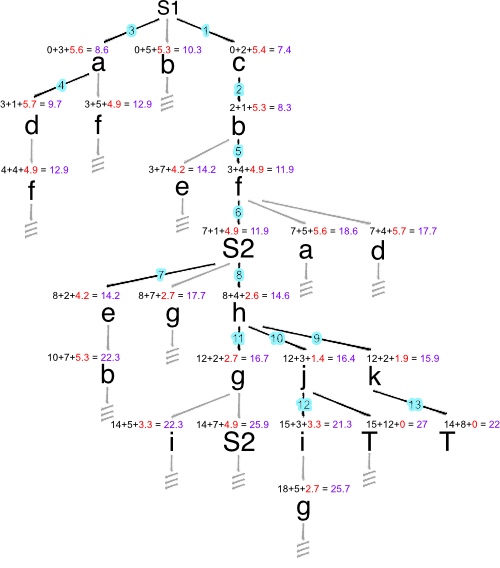
\includegraphics[scale=0.9]{chapters/informed_search/AStarBaum1.png}
	\caption{Such Baum B1 von T nach S1}
	\label{fig:searchtrees1}
\end{figure}

\begin{figure}[h!]
	\centering
	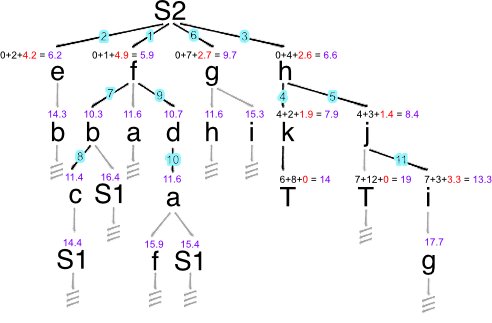
\includegraphics[scale=0.9]{chapters/informed_search/AStarBaum2.png}
	\caption{Such Baum B2 von T nach S2}
	\label{fig:searchtrees2}
\end{figure}
\newpage 
\chapterimage{chapter_head_1.png}

\chapter{Suchalgorithmen für Spiele}

\usetikzlibrary{arrows}
\usetikzlibrary{calc}
\usetikzlibrary{positioning}
\usetikzlibrary{matrix}

\pgfdeclarelayer{background}
\pgfsetlayers{background,main}

\tikzset{
    treenode/.style = {align=center, inner sep=0pt, text centered,
        font=\sffamily},
    arn_n/.style = {treenode, circle, white, font=\sffamily\bfseries, draw=blue, fill=blue,
        text width=1.5em, minimum width=1.5em, minimum height=1.5em},% arbre rouge noir, noeud noir
    arn_r/.style = {treenode, circle, white, draw=red, fill=red,
        text width=1.5em, very thick, minimum width=1.5em, minimum height=1.5em},% arbre rouge noir, noeud rouge
    arn_x/.style = {treenode, rectangle, draw=black,
        minimum width=1.5em, minimum height=1.5em},% arbre rouge noir, nil
}


\section{Intro \& Motivation}

In den vorangegangenen Kapiteln haben wir schon einige Suchverfahren kennengelernt, welche uns nun helfen werden Algorithmen zu verstehen, die verwendet werden um Computergegner für Nullsummenspiele zu entwickeln. Hierbei werden wir uns den Minimax-Algorithmus, sowie den Alpha-Beta-Algorithmus genauer anschauen, welche beide versuchen sich in die Lage des Gegners zu versetzen, um so  herauszufinden, welche Reaktion dieser auf einen Zug von uns wählen würde. Ziel der Algorithmen ist es, ein für uns bestmögliches Ergebnis und somit, wenn möglich, einen Sieg zu erlangen. Dieses Vorgehen kann eine Betrachtung von sehr vielen möglichen Züge zur Folge haben, was sehr viel Rechenaufwand bedeutet. Im Folgenden werden wir jedoch  mit Hilfe des Alpha-Beta-Algorithmus eine Methode kennenlernen, die es uns ermöglicht die Anzahl der zu betrachtenden Züge zu reduzieren.



\section{Inhaltliche Ausarbeitung des Themas}

Wir betrachten ein Nullsummenspiel, was bedeutet, dass der Gewinn des einen Spielers (Nutzwert positiv) mit dem Verlust des Gegners (Nutzwert negativ) äquivalent ist und ein Unentschieden keine Auswirkungen auf die Nullsummeneigenschaft hat (Nutzwert 0).
Gegeben sei für dieses Spiel ein Spielbaum $T = (V;E)$. Bei einem gleichförmigen Spielbaum besitzt jeder innere Knoten den gleichen Verzweigungsgrad b und alle Blätter befinden sich in der gleichen Tiefe d, sodass die Zahl der Knoten in einem gleichförmigen Baum exponentiell mit der Tiefe des Baumes wächst ($b^d$). Jedoch gibt es auch Spielbäume bei denen der Verzweigungsgrad der Ebenen variiert.
Der Spielbaum beinhaltet alle möglichen Züge und Spielausgänge. Die Tiefe und der Verzweigungsgrad hängt von dem Spiel ab, welches wir betrachten. Beispielsweise hat der Spielbaum zu einem Tic-Tac-Toe Spiel eine Tiefe von 9 (da es 9 Felder zu besetzen gibt) und zu Beginn des Spiels einen Verzweigungsgrad von 9 (weil noch alle 9 Felder zur Auswahl stehen), der mit wachsender Tiefe allerdings abnimmt, da nach jedem Zug immer ein leeres Feld weniger vorhanden ist.



\subsection{Problemstellung}
Zu dem gegebenen Nullsummenspiel wollen wir einen Computergegner programmieren, der in der Lage ist die optimale Antwort auf jede Spielposition, bei optimalem Spiel beider Spieler, zu finden.
Dafür müssen wir jedoch vorher festlegen, was für uns optimal in diesem Zusammenhang bedeutet. Wir gehen davon aus, dass der Gegner immer den für ihn optimalen Zug wählt, d.~h. den Zug, der für ihn zum besten Nutzwert und somit für uns zum schlechtesten Nutzwert führt. Analog wollen wir agieren. Wie dies genau funktioniert werden wir im folgenden Abschnitt sehen.



\subsection{Methoden}


\subsubsection*{Minimax Algorithmus}
Im folgenden bezeichnen wir unseren Spieler mit MAX und den gegnerischen Spieler mit MIN. Wie zuvor schon angedeutet ist das Ziel des Minimax-Algorithmus den Minimax-Wert für die aktuelle Stellung zu bestimmen. Der Minimax-Wert der Endstellungen (Blätter) entspricht dem Nutzwert für MAX. Die Berechnung der anderen Knoten erfolgt rekursiv mit Hilfe der folgenden Bewertungsfunktion:

\begin{center}
	$Minimax(k) = \begin{cases} Nutzwert(k) & \mathrm{falls}~k~\mathrm{Endzustand}\\
		max\{minimax(t) ~|~ t \in N(t)\} 	& \mathrm{falls}~k~\mathrm{MAX\hbox{-}Knoten}\\
		min\{minimax(t) ~|~ t \in N(t)\}	& \mathrm{falls}~k~\mathrm{MIN\hbox{-}Knoten}	\end{cases} $
\end{center}

wobei $N(t)$ die Funktion ist, die die Kinder im Baum liefert. Die Auswertung der Knoten geschieht Bottom up, das bedeutet wir beginnen bei den Blättern und bewerten von dort ausgehend die Elternknoten und anschließend deren Eltern bis wir irgendwann bei der Wurzel angelangt sind. Der Minimax Algorithmus liefert nicht unbedingt den höchsten Nutzwert der Blätter, sondern den größten Nutzwert den man erhalten kann, wenn der Gegner selbst versucht zu gewinnen und somit den Nutzwert für uns möglichst klein zu halten.\\

Anschaulicher wird das ganze, wenn man sich den Algorithmus an einem Beispiel anschaut.

\textbf{Beispiel}\\

Gegeben sei der folgende Spielbaum
\begin{center}
\includegraphics[width = 7 cm]{chapters/minimax/jpg/Graph-Minmax1.jpg}
\end{center}

Angenommen MIN wäre an der markierten Position:
\begin{center}
	\includegraphics[width = 7 cm]{chapters/minimax/jpg/Graph-Minmax2-1.jpg}
\end{center}

Dann würde MIN den Zug auswählen, der für ihn den größten Nutzwert und somit für uns den kleinsten Nutzwert hat. Das heißt in dem Fall:
\begin{center}
	 $min\{minimax(t) | t \in N(t)\} ~=~ min\{9,3\} ~=~ 3$

\includegraphics[width = 7 cm]{chapters/minimax/jpg/Graph-Minmax2-2.jpg}
\end{center}

Angenommen MIN wäre an der markierten Position:
\begin{center}
	\includegraphics[width = 7 cm]{chapters/minimax/jpg/Graph-Minmax2-3.jpg}
\end{center}

Dann würde MIN den Zug auswählen, der für ihn den größten Nutzwert und somit für uns den kleinsten Nutzwert hat. Das heißt in dem Fall:
\begin{center}
	$min\{minimax(t) | t \in N(t)\} ~=~ min\{1,5\} ~=~ 1$

	\includegraphics[width = 7 cm]{chapters/minimax/jpg/Graph-Minmax2-4.jpg}
\end{center}

Nun betrachten wir den Zug von MAX. Der Suchbaum sieht wie folgt aus

\begin{center}
	\includegraphics[width = 7 cm]{chapters/minimax/jpg/Graph-Minmax2.jpg}
\end{center}

MAX würde den Zug wählen, der für ihn den höchsten Nutzwert hat.\\

\begin{center}
	$max\{minimax(t) | t \in N(t)\} ~=~ max\{3,1\} ~=~ 3$
	\includegraphics[width = 7 cm]{chapters/minimax/jpg/Graph-Minmax3.jpg}
\end{center}

Somit sieht der Suchbaum nach Abschluss des Minimax-Algorithmus wie folgt aus, wobei der rote Pfad den optimalen Nutzwert liefert, wenn beide Spieler optimal spielen. Somit sollte MAX den linken Knoten wählen.

\begin{center}
	\includegraphics[width = 7 cm]{chapters/minimax/jpg/Graph-Minmax4.jpg}
\end{center}

\vskip 60pt



\subsubsection*{Problem:} Der Minimax-Algorithmus durchsucht den Suchbaum $T=(V, E)$ mit Tiefensuche, in der Zeit $O(max \{|V|, |E|\}) = O(|V|)$. Somit benötigt die Suche zwar lineare Zeit, jedoch wächst der Baum exponentiell mit zunehmender Tiefe ($O(|V|)=O(b^d)$). Somit ist der Algorithmus für Bäume mit großer Tiefe ineffizient.


\subsubsection*{Alpha-Beta-Algorithmus}
 Der Alpha-Beta-Algorithmus ist eine Verbesserung vom Minimax-Algorithmus, da die Zugriffsanzahl reduziert wird, indem Teile des Suchbaums nicht durchsucht werden, ohne dabei das Ergebnis zu verfälschen. Für die Umsetzung werden die Variablen $\alpha$ und $\beta$ eingeführt, wobei $\alpha$ der Nutzwert ist, welchen MAX mindestens erreicht und $\beta$ der Nutzwert, den MIN höchstens erreicht. Die Auswertung der Knoten geschieht on-the-fly, d.~h. nur dann, wenn wir sie wirklich benötigen. \\

 \underline{MAX-Knoten:}\\
 Betrachten wir einen MAX Knoten und stellen dort einen Wert fest, der größer ist als $\beta$, brauchen wir den Teilbaum nicht weiter betrachten, da MIN diesen nicht wählen würde, weil der andere Teilbaum einen kleineren Nutzwert liefert. Das nicht weiter Betrachten des Teilbaums bezeichnet man als Beta-Cutoff. Ist  der Wert des MAX Knoten größer als $\alpha$ erhöht sich der Wert den MAX mindestens erreicht und wir aktualisieren $\alpha$ auf den Wert des Knotens.  \\

 \underline{MIN-Knoten:}\\
 Ist der Wert eines MIN Knotens kleiner als der Wert von $\alpha$ müssen wir diesen Teilbaum nicht weiter analysieren, da MAX immer den Teilbaum mit dem größten Nutzwert auswählt und da $\alpha$ größer ist als der Wert des betrachteten Knotens existiert ein Teilbaum mit einem größeren Nutzwert. Also würde hier ein Cutoff stattfinden, welchen man als Alpha-Cutoff bezeichnet. Sollte jedoch der Wert des MIN Knotens größer als $\beta$ sein steigt der Wert den MIN höchstens erreicht und wir müssen $\beta$ auf diesen Wert anpassen.


 \begin{algorithm}
 	\KwData{Graph $G=(V,E)$, Blätter mit Nutzwert, s = Knoten}
 	\KwResult{Nutzwert für jeden knoten}
 	\textbf{alpha-beta-suche(s)}\\

 	\textbf{return} maximalerWert(s, -$\infty$, $\infty$)\\

 	\textbf{maximalerWert}(Knoten, $\alpha$, $\beta$)\\

	 	\If{s = Blatt}{
	 		\textbf{return} wert(s)
	 	}
	 	\Else{
	 		$wert = \alpha$\\
	 		\ForEach{k= Kind(s)}{
		 		$wert = max\{wert, minimalerWert(k, wert, \beta)\}$\\
		 		\If {$wert >= \beta$}{
			 		\textbf{return} wert}
			 	$\alpha = max\{\alpha, wert\}$\\
	 		}
			\textbf{return} wert
	 	}

	\textbf{minimalerWert}(Knoten, $\alpha$, $\beta$)\\

	\If{s = Blatt}{
		\textbf{return} wert(s)
	}
	\Else{
		$wert = \beta$\\
		\ForEach{k= Kind(Knoten)}{
			$wert = min\{wert, minimalerWert(k, \alpha, wert)\}$\\
			\If {$wert <= \alpha$}{
				\textbf{return} wert}
			$\beta = min\{\beta, wert\}$\\
		}
		\textbf{return} wert

	}
 	\caption{Alpha-Beta-Algorithmus}
\end{algorithm}

Betrachten wir ein Beispiel, um den Algorithmus besser zu verstehen.

\paragraph{Beispiel:}

Gegeben sei der folgender Spielbaum, blaue Knoten sind MAX- und rote MIN-Entscheidungen.
Wir folgen immer den linken Kindern. Zunächst treffen wir unsere erste Entscheidung, dafür müssen beide Kinder des linkesten Pfades evaluiert werden.
Wir entscheiden uns für die 5. Dieser Wert ist der neue $\beta$ -Wert für seinen Schwester-Knoten. Heißt unser Gegenspieler MIN wird sich höchstens für den Wert 5 entscheiden.

\begin{center}
\begin{tikzpicture}[->,>=stealth',level/.style={sibling distance = 5cm/#1,
    level distance = 1.5cm}]
\node [arn_n] {}
child{ node [arn_r] {}
    child{ node [arn_n] {5}
        child{ node [arn_x] {5}}
        child{ node [arn_x] {0}}
    }
    child{ node [arn_n] {}
        child{ node [arn_x] {}}
        child{ node [arn_x] {}}
        node[right = 1em]{$\beta=5$}
    }
}
child{ node [arn_r] {}
    child{ node [arn_n] {}
        child{ node [arn_x] {}}
        child{ node [arn_x] {}}
    }
    child{ node [arn_n] {}
        child{ node [arn_x] {}}
        child{ node [arn_x] {}}
    }
}
;
\end{tikzpicture}
\end{center}

Wir evaluieren den nächsten Knoten im Nachbar-Graphen. Er ist 6. Da dieser Wert größer-gleich des $\beta$-Wert ist, müssen wir den Rest des Teil-Graphen nicht zu evaluieren. Dies ist überflüßig, da MIN den tiefsten Wert wählen wird, welcher mindestens 5 ist. Wir brauchen also nicht nach einem noch größeren Wert suchen. \\
\textbf{Dies nennt man $\beta-Cut$.} \\
Der neue $\alpha$-Wert des roten Schwester-Konten ist nun 5. Heißt: Wir können danach mindestens eine 5 wählen.

\begin{center}
\begin{tikzpicture}[->,>=stealth',level/.style={sibling distance = 5cm/#1,
    level distance = 1.5cm}]
\node [arn_n] {}
child{ node [arn_r] {5}
    child{ node [arn_n] {5}
        child{ node [arn_x] {5}}
        child{ node [arn_x] {0}}
    }
    child{ node [arn_n] {6}
        child{ node [arn_x] {6}}
        child[dashed]{ node [arn_x] {}}
        node[right = 1em]{$\beta=5$}
    }
}
child{ node [arn_r] {}
    child{ node [arn_n] {}
        child{ node [arn_x] {}}
        child{ node [arn_x] {}}
    }
    child{ node [arn_n] {}
        child{ node [arn_x] {}}
        child{ node [arn_x] {}}
    }
    node[left = 1em]{$\alpha=5$}
}
;
\end{tikzpicture}
\end{center}

Da der ganze linke Teilbaum evaluiert ist, kann der rechte Baum evaluiert werden.
Dort wird wieder dem linkesten Pfad gefolgt. Wir evaluieren und setzen den $\beta$-Wert für den Schwesterknoten genauso wie im linken Teilbaum.

\begin{center}
\begin{tikzpicture}[->,>=stealth',level/.style={sibling distance = 5cm/#1,
    level distance = 1.5cm}]
\node [arn_n] {}
child{ node [arn_r] {5}
    child{ node [arn_n] {5}
        child{ node [arn_x] {5}}
        child{ node [arn_x] {0}}
    }
    child{ node [arn_n] {6}
        child{ node [arn_x] {6}}
        child[dashed]{ node [arn_x] {}}
        node[right = 1em]{$\beta=5$}
    }
}
child{ node [arn_r] {}
    child{ node [arn_n] {-1}
        child{ node [arn_x] {-1}}
        child{ node [arn_x] {-2}}
    }
    child{ node [arn_n] {}
        child{ node [arn_x] {}}
        child{ node [arn_x] {}}
        node[right = 1em]{$\beta=-1$}
    }
    node[left = 1em]{$\alpha=5$}
}
;
\end{tikzpicture}
\end{center}

Der Wert unserer letzten Entscheidung ist nun kleiner-gleich des nächsten $\alpha$-Werts. Dies bedeutet, dass unsere Seite des Graphens nicht mehr relevant ist. Wir (MAX) können mindestens eine 5 wählen. Der Gegner (MIN) wird allerdings in diesem Teil des Graphens höchstens eine -1 wählen. Wir brauchen den Rest des rechten Graphen also nicht weiter betrachten. \\
\textbf{Dies ist ein $\alpha-Cut$.}

\begin{center}
\begin{tikzpicture}[->,>=stealth',level/.style={sibling distance = 5cm/#1,
    level distance = 1.5cm}]
\node [arn_n] {5}
child{ node [arn_r] {5}
    child{ node [arn_n] {5}
        child{ node [arn_x] {5}}
        child{ node [arn_x] {0}}
    }
    child{ node [arn_n] {6}
        child{ node [arn_x] {6}}
        child[dashed]{ node [arn_x] {}}
        node[right = 1em]{$\beta=5$}
    }
}
child{ node [arn_r] {-1}
    child{ node [arn_n] {-1}
        child{ node [arn_x] {-1}}
        child{ node [arn_x] {-2}}
    }
    child[dashed]{ node [arn_n, fill=white] {}
        child{ node [arn_x] {}}
        child{ node [arn_x] {}}
    }
    node[left = 1em]{$\alpha=5$}
}
;
\end{tikzpicture}
\end{center}

Die gestrichelten Teile sind nun (mögliche) Teilgraphen, welche mit dem normalen MiniMax Algorithmus hätten evaluiert werden müssen. In diesem Beispiel haben wir 3/8 Blättern ignorieren können. Bei steigender Tiefe fallen so große Unterbäume weg.

\section{Abgrenzung / Vergleich zu den vorherigen Kapitel}

In den vorherigen Kapiteln haben wir verschiedene Suchalgorithmen (Bestensuche, Branch-and-Bound, A*) kennengelernt. Diese liefern den Pfad, der zu dem Blatt mit dem höchsten Nutzwert führt. Jedoch beachten sie nicht, ob der Gegner auch diesen Pfad wählen würde. Der Gegner würde versuchen den geringsten Nutzwert für uns zu erreichen und somit versuchen von diesem Pfad abzuweichen. Folglich würden sie keine realistische Einschätzung darüber geben, welche Züge das beste Spielergebnis liefern. Im Gegensatz dazu betrachten sowohl der Minimax, als auch der Alpha-Beta Algorithmus das Verhalten des Gegners, welches zu einer guten Einschätzung der Spielsituation führt.



\section{Fazit \& Bewertung}

Zusammenfassend lässt sich sagen, dass der Minimax- und der Alpha-Beta-Algorithmus zum selben besten Ergebnis für den MAX-Spieler führen und sich lediglich in ihrer Effizienz unterscheiden können, da der Alpha-Beta-Algorithmus weniger Berechnungen und somit eine kürzere Rechnungszeit benötigen kann. Je nach Suchbaum kann die Anzahl der Cutoffs und die Einsparung der Rechenzeit sehr groß ausfallen. Aufgrund dessen ist der Alpa-Beta-Algorithmus eine Grundlage für viele Algorithmen im Bereich der Nullsummenspiele für zwei Personen. Für die Berechnungen der Algorithmen sind die Werte der Blätter von größer Bedeutung, welche durch die Heuristik gegeben sind. Alles in allem kann man sagen, dass man sowohl mit Minimax als auch mit Alpha Beta einen Computergegner programmieren kann, der es einem Menschen sehr schwer, wenn nicht sogar unmöglich, macht zu gewinnen und somit eine künstliche Intelligenz bei Nullsummenspielen für die Zukunft denkbar ist.


\section{Quellen und Literatur}

\begin{itemize}
\item MIT - Lecture 6: Search: Games, Minimax, and Alpha-Beta
\item http://home.in.tum.de/~adorf/pub/alphabeta-seminar-paper.pdf
\item https://de.wikipedia.org/wiki/Minimax-Algorithmus
\item https://de.wikipedia.org/wiki/Alpha-Beta-Suche
\end{itemize}


\part{Lernende Systeme}
\include{chapters/svm/svm}
\include{chapters/neural_networks/networks}
\include{chapters/genetic/genetic}

\part{Sensorik \& Interaktion}
\include{chapters/computervision/cv}
\include{chapters/sprachverarbeitung/sprachverarbeitung}

\part{Philosophische Grundlagen}
\include{chapters/intelligenzbegriff/begriff}
\include{chapters/grenzen/grenzen}

\part{Appendix}

\defbibfilter{papers}{
  type=article or
  type=inproceedings
}

\chapter*{Literaturverzeichnis}
\addcontentsline{toc}{chapter}{\textcolor{hhublue}{Literaturverzeichnis}}
\section*{Bücher}
\addcontentsline{toc}{section}{Bücher}
\printbibliography[heading=bibempty,type=book]
\section*{Wissenschaftliche Artikel}
\addcontentsline{toc}{section}{Wissenschaftliche Artikel}
\printbibliography[heading=bibempty,filter=papers]
\section*{Webpages}
\addcontentsline{toc}{section}{Webpages}
\printbibliography[heading=bibempty,type=online]

%----------------------------------------------------------------------------------------
%	INDEX
%----------------------------------------------------------------------------------------

\cleardoublepage
\phantomsection
\setlength{\columnsep}{0.75cm}
\addcontentsline{toc}{chapter}{\textcolor{hhublue}{Index}}
\printindex

%----------------------------------------------------------------------------------------

\end{document}
